
\documentclass[review]{elsarticle}
\usepackage{comment}
\usepackage{url}
%
\usepackage[breaklinks]{hyperref}
\usepackage{breakurl}


\usepackage[ruled]{algorithm2e}

%\usepackage{lineno}
%\modulolinenumbers[5]

\journal{Optics \& Laser Technology}

%%%%%%%%%%%%%%%%%%%%%%%
%% Elsevier bibliography styles
%%%%%%%%%%%%%%%%%%%%%%%
%% To change the style, put a % in front of the second line of the current style and
%% remove the % from the second line of the style you would like to use.
%%%%%%%%%%%%%%%%%%%%%%%

%% Numbered
%\bibliographystyle{model1-num-names}

%% Numbered without titles
%\bibliographystyle{model1a-num-names}

%% Harvard
%\bibliographystyle{model2-names.bst}\biboptions{authoryear}

%% Vancouver numbered
%\usepackage{numcompress}\bibliographystyle{model3-num-names}

%% Vancouver name/year
%\usepackage{numcompress}\bibliographystyle{model4-names}\biboptions{authoryear}

%% APA style
%\bibliographystyle{model5-names}\biboptions{authoryear}

%% AMA style
%\usepackage{numcompress}\bibliographystyle{model6-num-names}

%% `Elsevier LaTeX' style
\bibliographystyle{elsarticle-num}
%%%%%%%%%%%%%%%%%%%%%%%
\usepackage{graphicx}
\usepackage{subcaption}
%%%%%%%%%%%%%%%%%%%%%%%%%%%%%%%%%%%%%%%%%%%%%%%%%%%%%%%%%%%%%%%%%%%%%%%%%%%%%%%%%%

\usepackage[svgnames]{xcolor} % Enabling colors by their 'svgnames'

\usepackage{amsmath}
\usepackage{amsfonts}
\usepackage{amssymb}
%%%%%%%%%%%%%%%%%%%%%%%%%%%%%%%%%%%%%%%%%%%%%%%%%%%%%%%%%%%%%%%%%%%%%%%%%%%%%%%%%%

 
\begin{document} 

\begin{frontmatter}

\title{Study of Illumination Dependency  in the Dynamic Laser Speckle Analysis}
%\tnotetext[mytitlenote]{Fully documented templates are available in the 
%elsarticle package on \href{http://www.ctan.org/tex-archive/macros/latex/contrib/elsarticle}{CTAN}.}



% Group authors per affiliation:
\author{Fernando Pujaico Rivera}
\author{Roberto Alves Braga Jr.}



\address{University Federal of Lavras, Lavras, Brazil}
\fntext[myfootnote2]{201518201@posgrad.ufla.br}
\fntext[myfootnote1]{robertobraga@deg.ufla.br }
% 


\begin{abstract}
In this article we show an analysis of how the frequency bands 
influence in the light independence of the speckle index value in a dynamic laser speckle analysis. 
Specifically, 
we studied temporal speckle deviation 
index influenced by the use of three different frequency bands of the speckle signal. 
Finally, it was shown how signals with high frequency components return values with greater illumination level independence.
\end{abstract}

\begin{keyword}
Biospeckle laser \sep 
Biospeckle index \sep 
Biospeckle signal\sep 
Biological activity \sep
Dynamic speckle 
\end{keyword}

\end{frontmatter}

\linenumbers

%%%%%%%%%%%%%%%%%%%%%%%%%%%%%%%%%%%%%%%%%%%%%%%%%%%%%%%%%%%%%%%%%%%%%%%%%%%%%%%%%%%%%%%%%
%%%%%%%%%%%%%%%%%%%%%%%%%%%%%%%%%%%%%%%%%%%%%%%%%%%%%%%%%%%%%%%%%%%%%%%%%%%%%%%%%%%%%%%%%
\section{Introduction}
Dynamic laser speckle is a phenomenon that is used to monitor changes in laser illuminated samples, and it can be measured by multiple indexes \cite{BSLTLBOOK}. The indexes are associated to the level of changes and could be expressed by numerical and or graphical outcomes that can be affected by filtering action during the image processing \cite{RIVERA2017144}. As an example, we have  the $AVD$ \cite{avd} and 
$IM$ \cite{ARIZAGA1999163} indexes, that filter
the information present in the history of the speckle images like a first order high pass filter with a cut-off in the middle
of the normalized frequency band. 
For this reason, it is important to analyze how
the chosen frequency band alters the result of selected index.
By other side, there is still a limitation to make speckle analysis in the presence of non homogeneous illumination, because
the most of biospeckle indexes are influenced in their values
by the use of an specific illumination level \cite{REIS2016}.
The illumination level can vary regarding the profile of the sample, such as an apple \cite{KAZ:12a} or a very irregular surface present in a kefir \cite{kefir}. 
It can also vary in accordance with the moisture present in the seed \cite{CARDOSO2011} due to the penetration of the light in the sample, or even when the color of the sample vary such as in the interface of cancer and normal tissues \cite{BCB+:12a}. And that is the reason to a continuous search for an adequate index, despite the fact there are many of them present in literature \cite{BSLTLBOOK}, but still without a solution to the independence of light intensity. 
The movement toward the portable equipment \cite{Bra:17}, reinforce the need to search the methods and its relation with the illumination. 
Thus, the present work aimed to establish a relation between the frequency band used
and the speckle index; particularly in the dependence of
the temporal speckle deviation matrix \cite{Nothdurft:05} with the illumination level.


%%%%%%%%%%%%%%%%%%%%%%%%%%%%%%%%%%%%%%%%%%%%%%%%%%%%%%%%%%%%%%%%%%%%%%%%%%%%%%%%%%%%%%%%%
%%%%%%%%%%%%%%%%%%%%%%%%%%%%%%%%%%%%%%%%%%%%%%%%%%%%%%%%%%%%%%%%%%%%%%%%%%%%%%%%%%%%%%%%%
\section{System description}
\label{sec:description}

\subsection{Data packages of ink drying}
\label{sec:descriptionink}
Fig. \ref{fig:system} shows the system setup of the ink sample test during drying where
a red laser was pointed to a layer of ink drying monitored by a digital camera;
the images are collected receiving two different illumination levels, 
because the neutral density lens partially covers partially the laser beam \cite{REIS2016}.
The images were placed in data packages and
are sampled with a time rate acquisition of $F_s=$ 12.5 hertz, being 
collected $N=400$ images by package. In total were collected $11$ packages 
(with the two different illumination levels each one) at the minutes 
$0$, $10$, $20$, $30$, $40$, $50$, $60$, $75$,$105$,$120$ and $150$ of drying process. 
\begin{figure}[ht!]
\centering
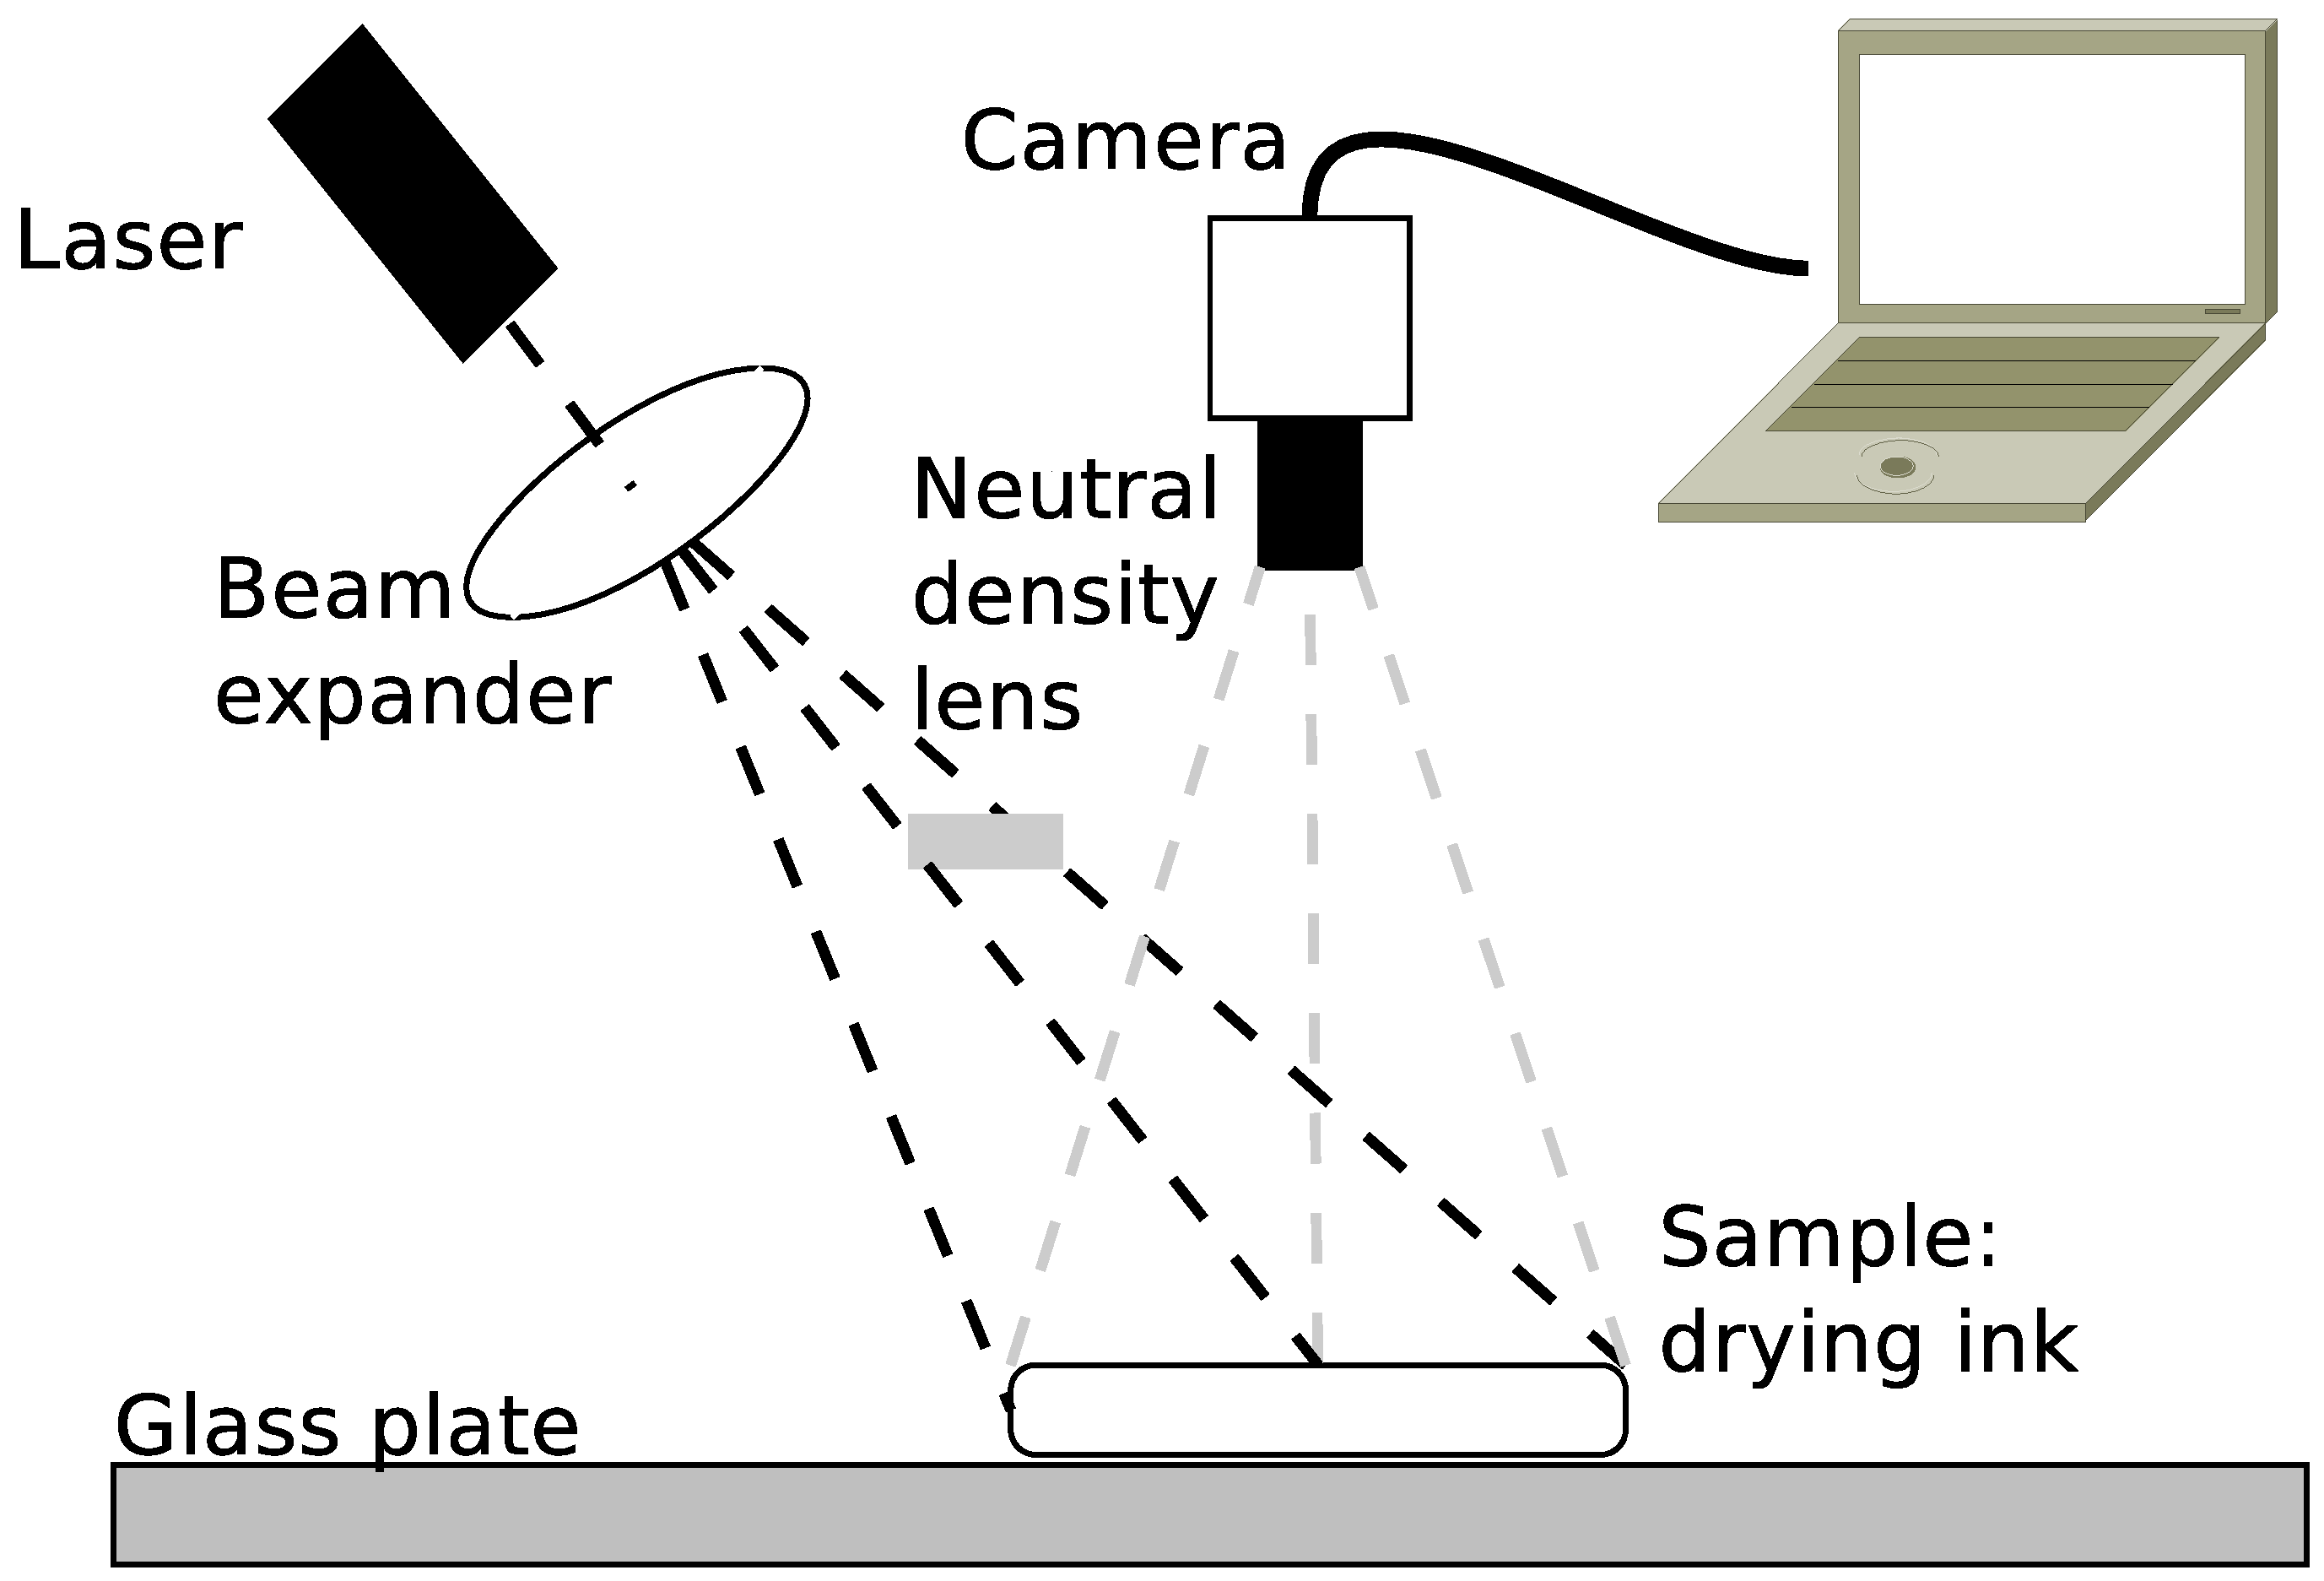
\includegraphics[width=0.65\columnwidth]{system.eps}
\caption{Experimental configuration of dynamic laser speckle formation monitored by digital system 
with the levels of illumination over a layer of ink drying.}
\label{fig:system}
\end{figure}
In each image of the packages were selected two regions, of $250\times200$ pixels, 
corresponding to the regions with two different illumination levels, 
as shown with red lines in the Fig. \ref{fig:regions}; thus, 
in the right side of the Fig. \ref{fig:regions}  we have the
portion of image that was altered by the neutral density lens.
Thus, the right side has low illumination, and
the left side has a high illumination.
\begin{figure}[h!]
\centering
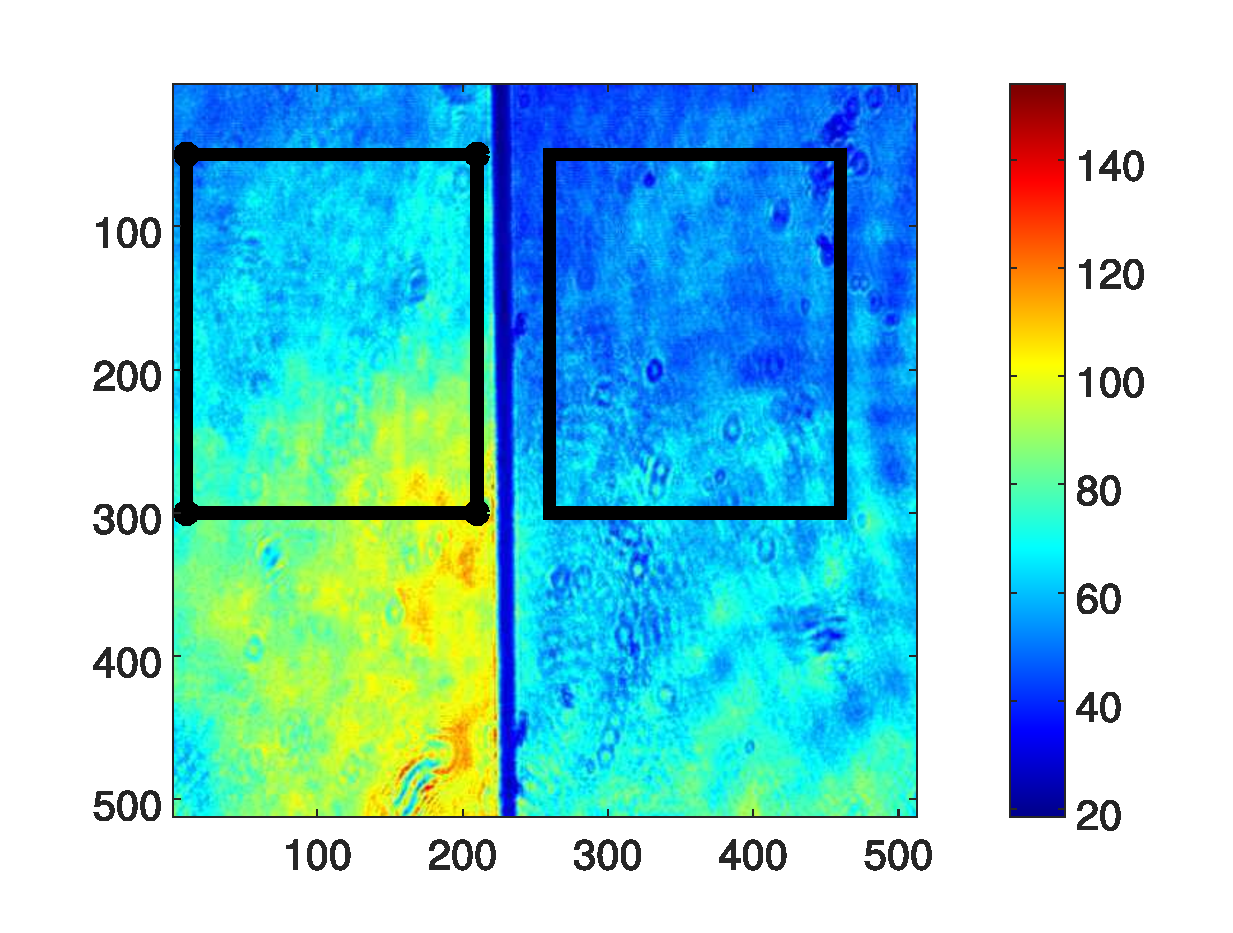
\includegraphics[width=0.85\columnwidth]{meanall_points_all.eps}
\caption{Selected regions and light intensity distribution in the ink drying test.}
\label{fig:regions}
\end{figure}
%\textcolor{red}{Nesta figura 2 poderíamos colocar também as imagens cruas dos padrões de speckle}\\

\subsection{Data packages of a steady state paper}
\label{sec:descriptionpaper}
The test over a steady state paper has a similar configuration that seen in
the Fig. \ref{fig:system} with the absence of 
the neutral density lens. 
The phenomenon observed was the speckle signal  variation associated with  the speckle response of material, 
the experimental setup of the camera, the resolution of the images and also to the mechanical noise; 
so that it was collected one data package sampled with a frequency of $F_s=$ 10 hertz, being 
collected in total $N=129$ images of 640$\times$480 pixels.
The Fig. \ref{fig:meanpaper} represents
with a color bar the result of  calculus the temporal speckle mean matrix ($\mu$) according the Eq. (\ref{eq:cont1})
showed in the Sec. \ref{subsec:deviation}; thus, it is easy to see how the
illumination level of laser over the paper has an elliptical form being highest 
close to the top of the image.
\begin{figure}[h!]
\centering
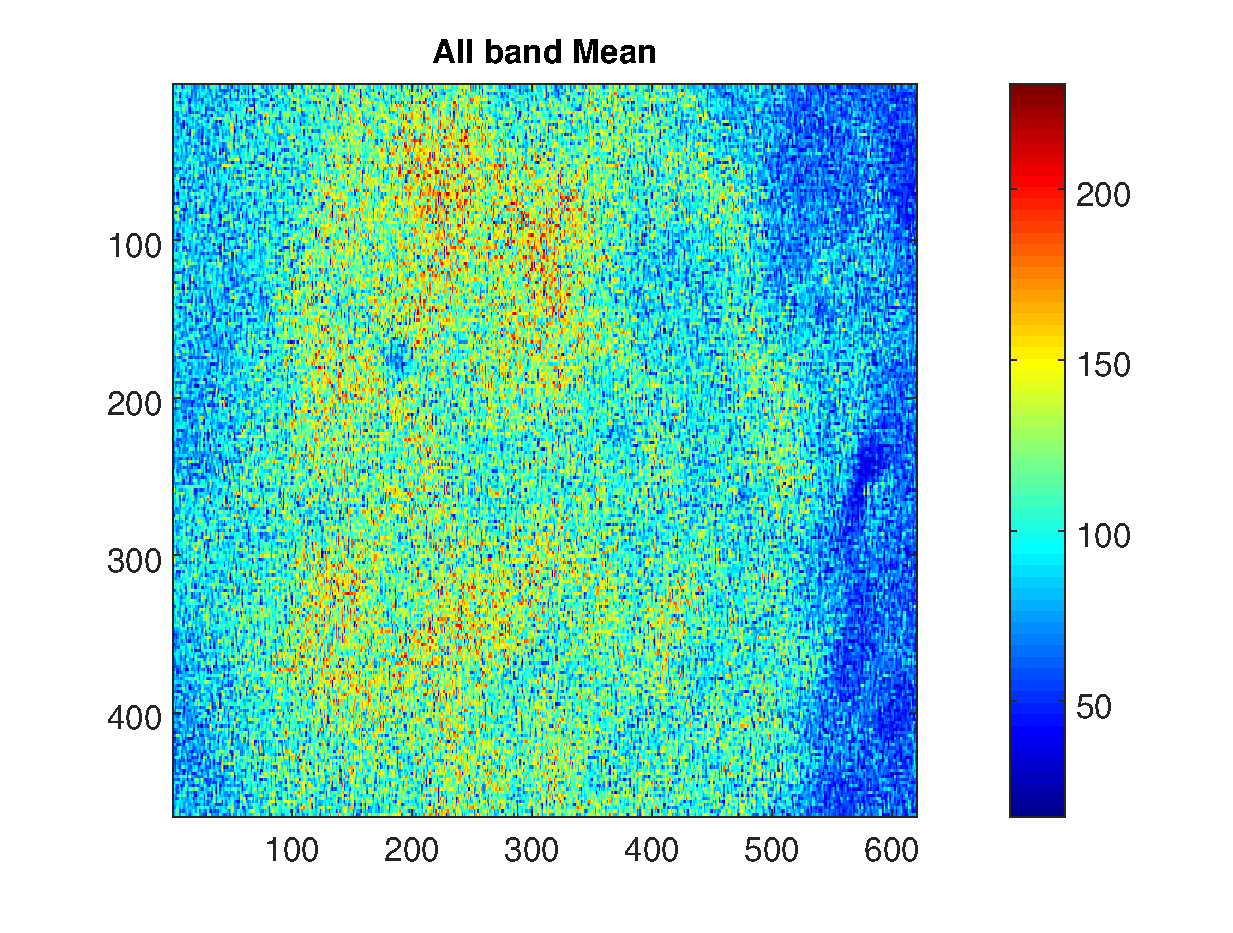
\includegraphics[width=0.85\columnwidth]{meanall.eps}
\caption{Light intensity distribution in the paper piece test with highest illumination 
presented by red pixels and lowest by blue pixels.}
\label{fig:meanpaper}
\end{figure}

%%%%%%%%%%%%%%%%%%%%%%%%%%%%%%%%%%%%%%%%%%%%%%%%%%%%%%%%%%%%%%%%%%%%%%%%%%%%%%%%%%%%%%%%%
%%%%%%%%%%%%%%%%%%%%%%%%%%%%%%%%%%%%%%%%%%%%%%%%%%%%%%%%%%%%%%%%%%%%%%%%%%%%%%%%%%%%%%%%%
\section{Numerical analysis}
\label{sec:analysis}

The sampling frequency used in the analysis of each test, 
it was selected  trying to achieve the best speed of sampling to observe each phenomenon. 
The purpose of these two tests is to observe the behavior of the indices in two cases; 
one with an activity homogeneous level in space and time, and another with a heterogeneous activity.
Thus, given that the paper activity test and the ink drying test are independent events, 
without comparison between them self, your sampling frequencies are different,
and selected according to the best behavior of the curves, 
being more appropriate higher sampling frequencies for the ink drying test.

\subsection{Data package filtering in three frequency band}
\label{subsec:firfilters}
Each data package or sub package ($P_T$) went through of a filter bank with 4 outputs  having each
one, a different type of processing, the first output is trivial because it
lets to pass the information freely, this package is called of $P_T$, whilst the other 3 outcomes
return  signals filtered by a frequency band; thus, 
we have the band between $[0,\frac{1}{3}]\frac{F_s}{2}$ (low frequencies),
the band between $[\frac{1}{3},\frac{2}{3}]\frac{F_s}{2}$ (intermediate frequencies) and
the band between $[\frac{2}{3},1]\frac{F_s}{2}$ (high frequencies); obtaining at end, the packages 
$P_X$, $P_Y$ and $P_Z$, respectively; as can be seen in the  Fig. \ref{fig:firfilters}.
The filtered packages of images were carried out using cascades
of two low-pass Finite Impulse Response ($FIR$) filters of order $32$, so that
the sum of signals $P_X+P_Y+P_Z=P_T$.
\begin{figure}[h!]
\centering
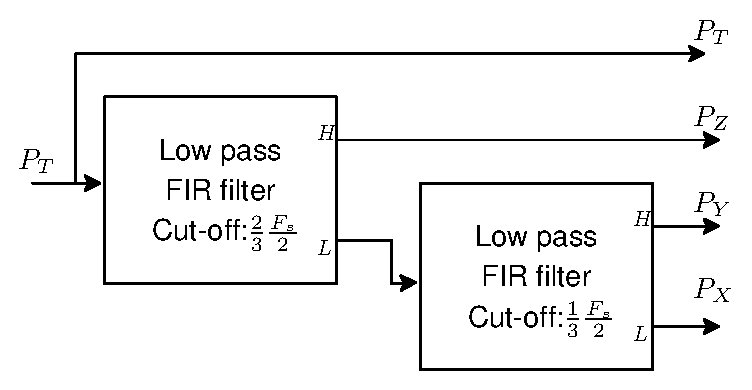
\includegraphics[width=0.55\columnwidth]{firfilters.eps}
\caption{Filtering of data packages.}
\label{fig:firfilters}
\end{figure}



\subsection{Temporal speckle deviation matrix}
\label{subsec:deviation}
The temporal speckle deviation matrix ($\sigma$) \cite{Nothdurft:05},
used to compare the results, it was obtained from the $N$ images of the data package $P$.
We designate to each image matrix, in the package $P$, as $\mathbf{I}_{k}$, $1\leq k \leq N$, 
being $k$ an integer index that indicates that, it is in use the $k$-th image $\mathbf{I}$ in the package.
Thus, to get
% the value $\bar{\sigma}$, it is necessary to get 
the matrix $\sigma$ is used the Equation \ref{eq:cont2}, 
\begin{equation}\label{eq:cont2}
\sigma  = \sqrt{ \frac{1}{N} \sum_{k=1}^{N} (\mathbf{I}_{k}-\mu)^2  },
\end{equation}
being that, the matrix $\mu$ can be calculated as, 
\begin{equation}\label{eq:cont1}
\mu =  \frac{1}{N} \sum_{k=1}^{N} \mathbf{I}_{k}.
\end{equation}
In these last two equations, all the operations are matricial, 
so that each element (aka pixel) $\mathbf{I}_{k}(i)$ in the matrix $\mathbf{I}_{k}$
should be processed with your  counterpart $\mathbf{I}_{k+1}(i)$ in the matrix $\mathbf{I}_{k+1}$.


Aditionally, the temporal speckle deviation index can be defined as $\bar{\sigma}=<\sigma>$, the mean value
of all elements in the matrix $\sigma$, being $<.>$ the mean spatial operator.
%And $\sigma_p$ as any value of an element in  $\sigma$.


\subsection{Fujii matrix}
\label{subsec:fujii}

The Fujii matrix \cite{Fujii:87} is obtained from the $N$ images in the data package $P$.
Similarly to the Section \ref{subsec:deviation}, 
we designate to each image matrix, in the package $P$, as $\mathbf{I}_{k}$, $1\leq k \leq N$.
Thus, to get the Fujii matrix is used the Equation \ref{eq:contFujii2}, 
\begin{equation}\label{eq:contFujii2}
Fujii  = \frac{1}{N-1} \sum_{k=1}^{N-1} \frac{|\mathbf{I}_{k}-\mathbf{I}_{k+1}|}{\mathbf{I}_{k}+\mathbf{I}_{k+1}}.
\end{equation} 
The  Fujii matrix mean value can be defined as $\overline{Fujii}=<Fujii>$, the mean value
of all elements in the $Fujii$ matrix.

The Fujii method represents the attempt to eliminate 
the dependence on illumination level, in a speckle index.
For this purpose, the method define the index as the mean value of the  first order high pass FIR filter, 
$\mathbf{I}_{k}-\mathbf{I}_{k+1}$, similarly to the  $AVD$ index \cite{avd};
but in the Fujii method the values are corrected using an approximation of the intensity mean value, 
$\frac{\mathbf{I}_{k}+\mathbf{I}_{k+1}}{2}$.
This calculation aspect is the strong point of the method,
because the method assumes that the increase in the speckle 
light dynamic range ($\mathbf{I}_{k}-\mathbf{I}_{k+1}$) 
will be linear in proportion with the increase in laser light ($\frac{\mathbf{I}_{k}+\mathbf{I}_{k+1}}{2}$).
This means that the method already uses high frequency components, 
of the speckle signal, 
and discards those of low frequency, 
in addition to attempting to correct or  normalize the index values;
and it is for these characteristics that it shows an acceptable performance,
to eliminate or decrease the dependence of the index with the laser intensity level.

Additionally, it was defined the matrix $Fujii_{\alpha}$, 
as the index of the filtered version of package $P$ to the frequency band $\alpha$, following the Equation \ref{eq:contFujii3}.
\begin{equation}\label{eq:contFujii3}
Fujii_{\alpha}  = \frac{1}{N-1} \sum_{k=1}^{N-1} \frac{|\mathbf{(I_{\alpha})}_{k}-\mathbf{(I_{\alpha})}_{k+1}|}{\mathbf{I}_{k}+\mathbf{I}_{k+1}}.
\end{equation}
It is important to highlight that the numerator of the last equation, 
use the signal in the matrices $\mathbf{(I_{\alpha})}_{k}$, that are filtered versions in the frequency band $\alpha$,
of the matrix $\mathbf{I}_{k}$. 
By other side, the denominator use the signal $\mathbf{I}_{k}$ which has the complete frequency band.
This modification was implemented because the numerator, in the calculus, 
represents or try be the mean value of speckle light intensity, 
and it value tend to zero in frequency bands without 0 hertz components.


\subsection{Datapack processing in the ink drying test}
\label{subsec:numprocink}

We have in the ink drying regions
two levels of illumination; thus, we  separated each package in two sub package
(high and low illumination), representing each one of the regions shown in the Fig. \ref{fig:regions}.
These sub-packages were filtered,
obtaining the packages $P_T$, $P_X$, $P_Y$ and $P_Z$, that was used to obtain
\begin{figure}[h!]
\centering
\includegraphics[width=0.65\columnwidth]{filtering.eps}
\caption{Filtering of data packages.}
\label{fig:filtering}
\end{figure}
the temporal speckle deviation matrix and the 
temporal speckle deviation indexes $\bar{\sigma}_T$, $\bar{\sigma}_X$, $\bar{\sigma}_Y$ and
$\bar{\sigma}_Z$.

\subsection{Statistical analysis of relation between the matrices $\sigma$ and $\mu$}
\label{subsec:statistical}
We define $\sigma_i$ and $\mu_i$
as the values in the $i-th$ position in the $\sigma$  
and $\mu$ matrices, respectively; we also defined $\mu_p$
as any element value in  $\mu$.
And we define the set $S_{\mu_p}=\{\sigma_i: \mu_i\equiv \mu_p; \forall i\}$
as the set of all $\sigma_i$  values given that $\mu_i\equiv\mu_p$.
Then, we obtained the vectors $L_p$, $\sigma_p$ and
$e_p$ using all the $\mu_p$ values, according to:
\begin{itemize}
 \item $L_p(\mu_p)=card\left(S_{\mu_p}\right)$,  being $L_p(\mu_p)$ the number of elements
 in the set $S_{\mu_p}$ and $card(.)$ the cardinality function operator.
 \item $\sigma_p(\mu_p)=mean\left(S_{\mu_p}\right)$, being $\sigma_p(\mu_p)$
 the mean value of elements in the set $S_{\mu_p}$ with $mean(.)$ representing the mean value function operator.
 \item $e_p(\mu_p)=std\left(S_{\mu_p}\right)$, being $\e_p(\mu_p)$
 the standard  deviation value of elements in the set $S_{\mu_p}$ with $std(.)$ representing the standard deviation function operator.
\end{itemize}
In practice only will be taken the vectors, values of $\mu_p$
with a $L_p(\mu_p)>200$ samples, to establish a limit to consider a set of representative samples.


\subsection{Datapack processing in the steady state paper test}
\label{subsec:numprocink}

In this test we have one data package that was filtered (\ref{fig:filtering2}) 
obtaining the packages $P_T$, $P_X$, $P_Y$ and $P_Z$, where the outcomes are the temporal speckle mean matrix and the 
temporal speckle deviation matrix, as can be seen in the Fig. \ref{fig:filtering2}.

\begin{figure}[h!]
\centering
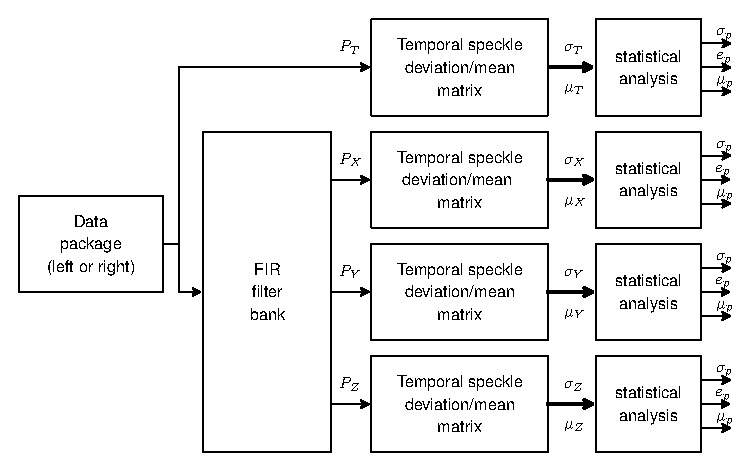
\includegraphics[width=0.65\columnwidth]{filtering2.eps}
\caption{Filtering of data package in the steady paper obtaining the mean and the deviation outcomes.}
\label{fig:filtering2}
\end{figure}




%%%%%%%%%%%%%%%%%%%%%%%%%%%%%%%%%%%%%%%%%%%%%%%%%%%%%%%%%%%%%%%%%%%%%%%%%%%%%%%%%%%%%%%%%
%%%%%%%%%%%%%%%%%%%%%%%%%%%%%%%%%%%%%%%%%%%%%%%%%%%%%%%%%%%%%%%%%%%%%%%%%%%%%%%%%%%%%%%%%
\section{Numerical results} 
\label{sec:numerical}


In the analysis, the minimum grayscale value, 
it is fixed by the observable minimum light by the camera or the minimum speckle light intensity in the material analyzed.
By other side, the maximum grayscale value, 
it is fixed by the observable maximum light by the camera or the maximum speckle light intensity in the material analyzed.

\subsection{Numerical results in the ink drying test} 
\label{subsec:numericalink}

The activity level analysis in the ink drying process has as objective to analyze 
the behavior of speckle index in a  dynamic process,
in the context of a system that change your characteristic in time. 

In the Fig. \ref{fig:numerical}, we can see the result of processing 
 the ink drying test under the dynamic laser speckle index (DLSI) in two areas with 
different level of illumination. The Fig. \ref{fig:allink}
represents the $\bar{\sigma}_T$ value in two light intensity levels, and it is done using the package $P_T$
trough the time, with the complete frequency bands.
The Fig. \ref{fig:stdxink}
represents the $\bar{\sigma}_X$ value in two light intensity levels, an it is done using the package $P_X$
trough the time, with the frequency band between $0$ and $\frac{1}{3}\frac{F_s}{2}$Hz.
The Fig. \ref{fig:stdyink}
represents the $\bar{\sigma}_Y$ value in two light intensity levels, and it is done using the package $P_Y$
trough the time, with the frequency band between $\frac{1}{3}\frac{F_s}{2}$ and $\frac{2}{3}\frac{F_s}{2}$ Hz.
And the Fig. \ref{fig:stdzink}
represent the $\bar{\sigma}_Z$ value in two light intensity levels, and it is done using the package $P_Z$
trough the time, with the frequency band between $\frac{2}{3}\frac{F_s}{2}$ and $\frac{F_s}{2}$ Hz.
\begin{figure}[h!]
    \centering
    \begin{subfigure}[b]{0.475\textwidth}
        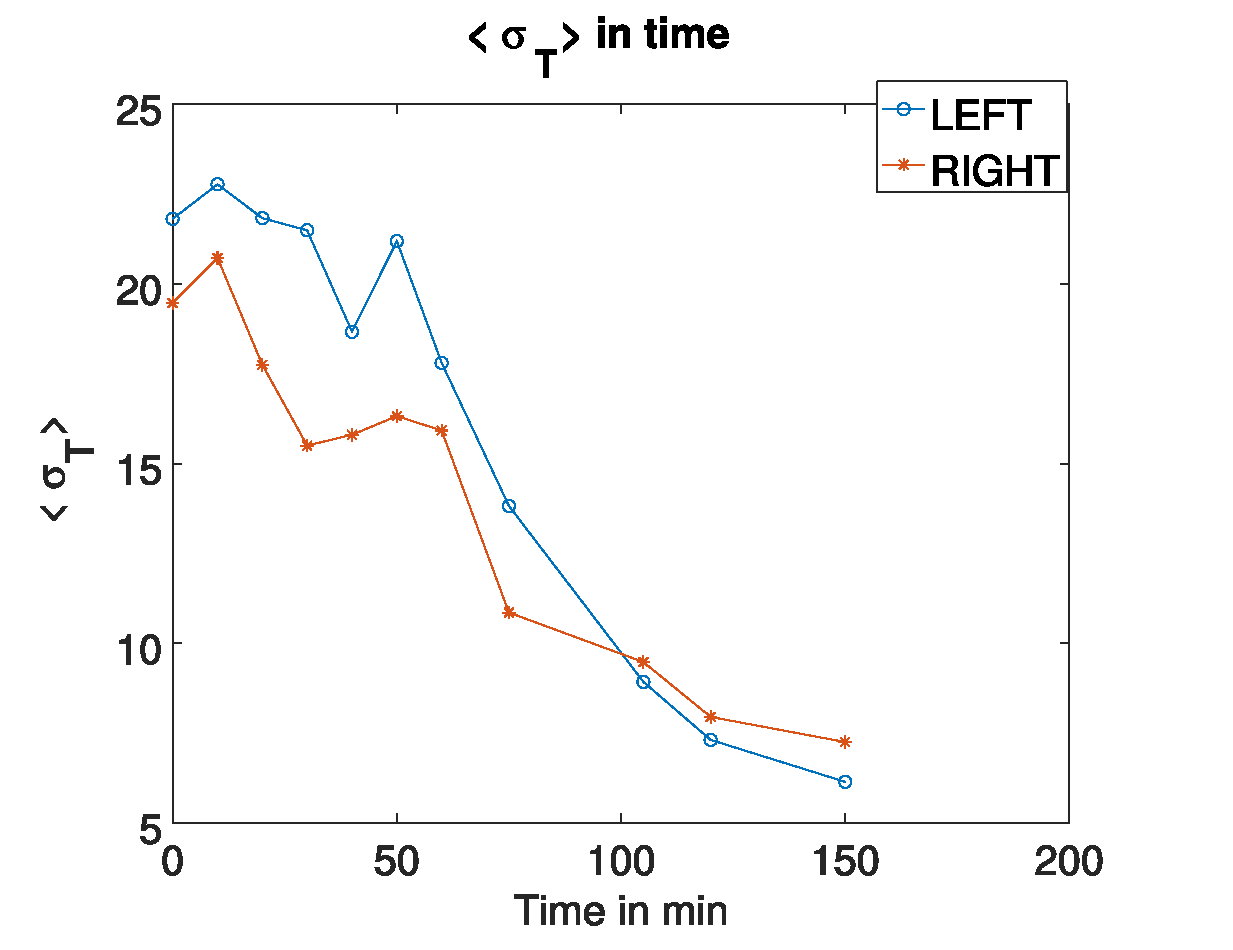
\includegraphics[width=\textwidth]{std-all.eps}
	\caption{$\bar{\sigma}_T$ value through  the time.}
        \label{fig:allink}
    \end{subfigure}
    ~
    \begin{subfigure}[b]{0.475\textwidth}
        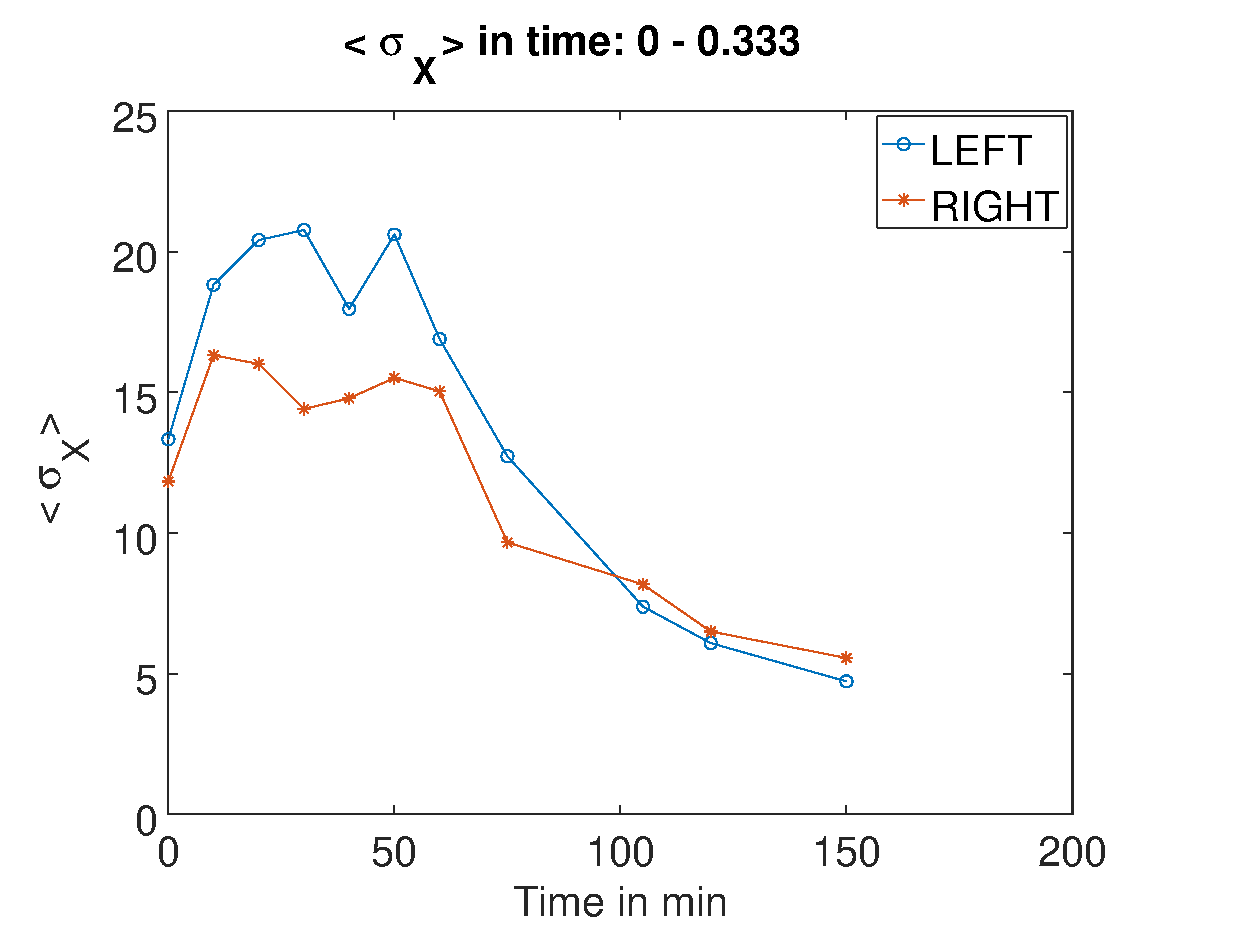
\includegraphics[width=\textwidth]{std-bandx.eps}
	\caption{$\bar{\sigma}_X$ value through  the time.}
        \label{fig:stdxink}
    \end{subfigure}
    ~\\ 
    \begin{subfigure}[b]{0.475\textwidth}
        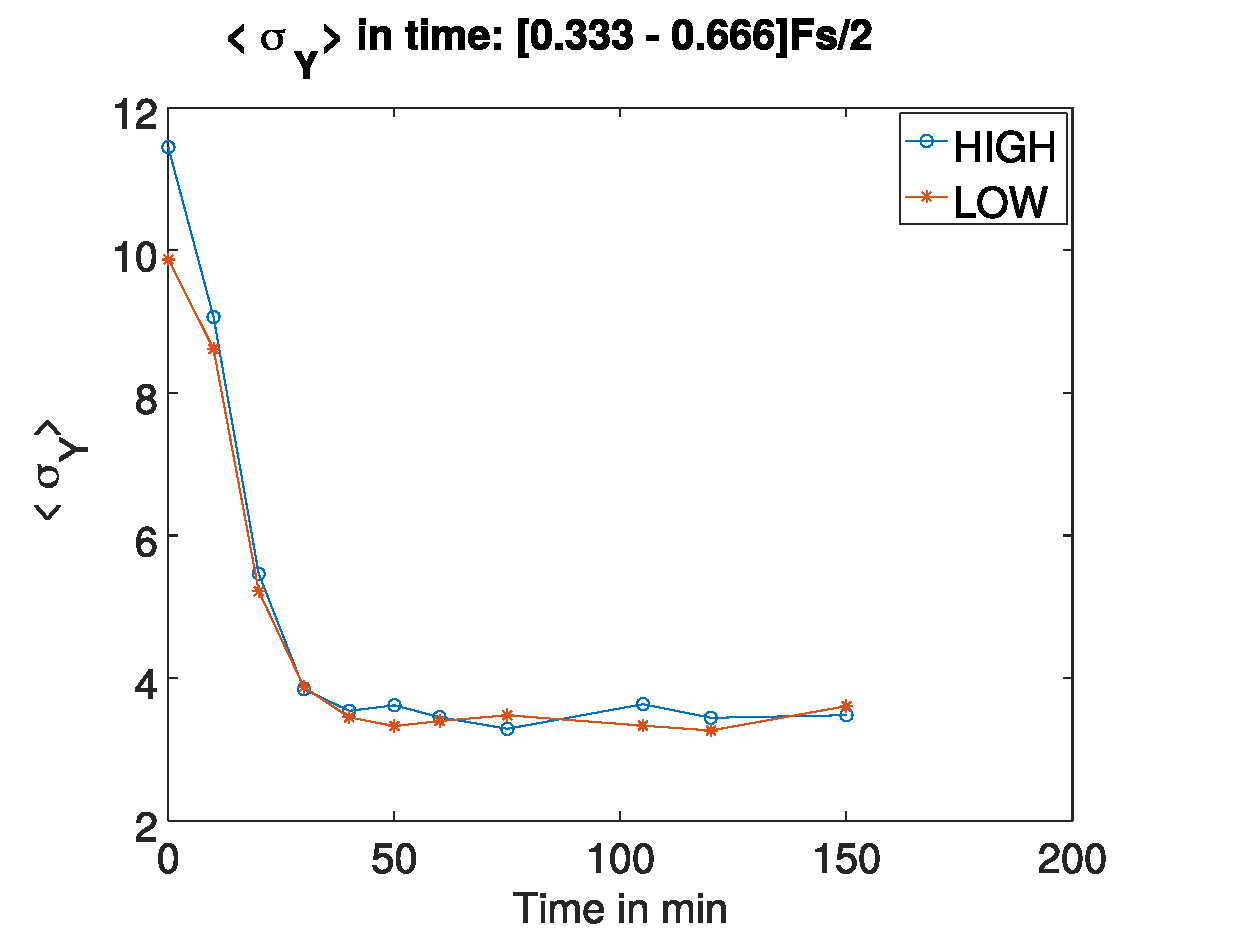
\includegraphics[width=\textwidth]{std-bandy.eps}
	\caption{$\bar{\sigma}_Y$ value through  the time.}
        \label{fig:stdyink}
    \end{subfigure}
  ~
    \begin{subfigure}[b]{0.475\textwidth}
        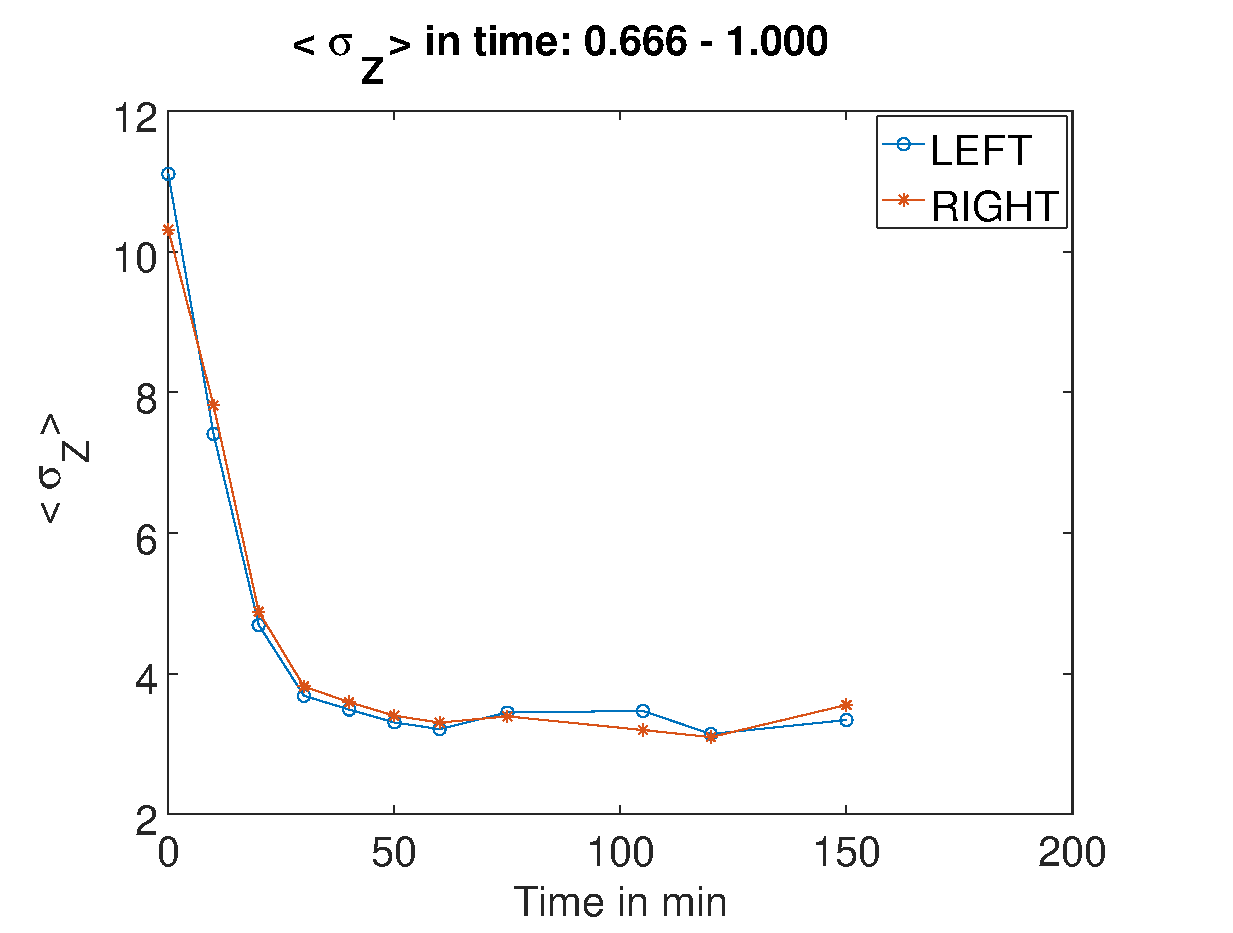
\includegraphics[width=\textwidth]{std-bandz.eps}
	\caption{$\bar{\sigma}_Z$ value through  the time.}
        \label{fig:stdzink}
    \end{subfigure}
    
\caption{Numerical results in the ink drying test.}\label{fig:numerical}
\end{figure}

As can be seen, when we analyzed the index over the complete frequency band (Fig. \ref{fig:allink}),
we had different results to both illuminations levels, being high in the left 
side of the Fig. \ref{fig:regions} and low in the right. This 
indicates a positive influence of illumination level in the index value.
By other side, if we observe the Figs. \ref{fig:stdxink}, \ref{fig:stdyink} and \ref{fig:stdzink},
we can see how the index values from different illuminations were similar when compared at the same frequency component,
being greatest similarity in the frequency band between $\frac{2}{3}\frac{F_s}{2}$ and $\frac{F_s}{2}$ Hz.

Finally, it is important to highlight that in the ink drying test, the information 
from the dynamic laser speckle is linked to high frequencies in the beginning of 
the drying process and  speckle signals with low frequencies at end, being gradual the transition
until reach the lowest level of signal with only the speckle signal of glass plate.
In Fig. \ref{fig:numerical} ($c-d$) one can see that after 50 minutes there is a 
transition of state with the stabilization of the DLSI. Thus, after this point, 
one has only the glass plate speckle signal influencing the DLSI.

This indicates that the comparisons of index illumination independence
only should be made between the first minutes because out this range we will be using high contribution of 
the noise as outcome.

\subsection{Numerical results of a steady paper under laser light} 
\label{subsec:numericalpaper}

%The paper piece test has a quasi-circular laser light distribution around a center and with decreasing 
light intensity with increasing the radius.

Even if the activity level of a paper piece, 
it  is considered as noise in the context of other tests, where takes place over it, 
a process of greater activity and variant in time and space. 
The speckle signal analysis of a paper piece, 
that for this test we consider approximately homogeneous in its characteristics over time and space,
will show us  the variation effect of an unique parameter, the light intensity on the dynamic speckle analysis.

In the Fig. \ref{fig:papelstd} we can see the result of data processing from the steady
 paper under dynamic laser speckle phenomenon, 
considering an homogeneous behavior of the speckle signal and using the standard deviation $\sigma$ 
as a dynamic laser speckle index (DLSI). 
Fig. \ref{fig:papelall} represents the $\sigma_T$ matrix with the complete frequency band, while Fig. \ref{fig:papelstd_stdx}
represents the $\sigma_X$ matrix with the frequency band between $0$ and $\frac{1}{3}\frac{F_s}{2}$Hz.
Fig. \ref{fig:papelstd_stdy} represents the $\sigma_Y$ matrix with the frequency band between 
$\frac{1}{3}\frac{F_s}{2}$ and $\frac{2}{3}\frac{F_s}{2}$ Hz, and Fig. \ref{fig:papelstd_stdz} 
represents the $\sigma_Z$ matrix with the frequency band between $\frac{2}{3}\frac{F_s}{2}$ and $\frac{F_s}{2}$ Hz.
\begin{figure}[h!]
    \centering
    \begin{subfigure}[b]{0.485\textwidth}
        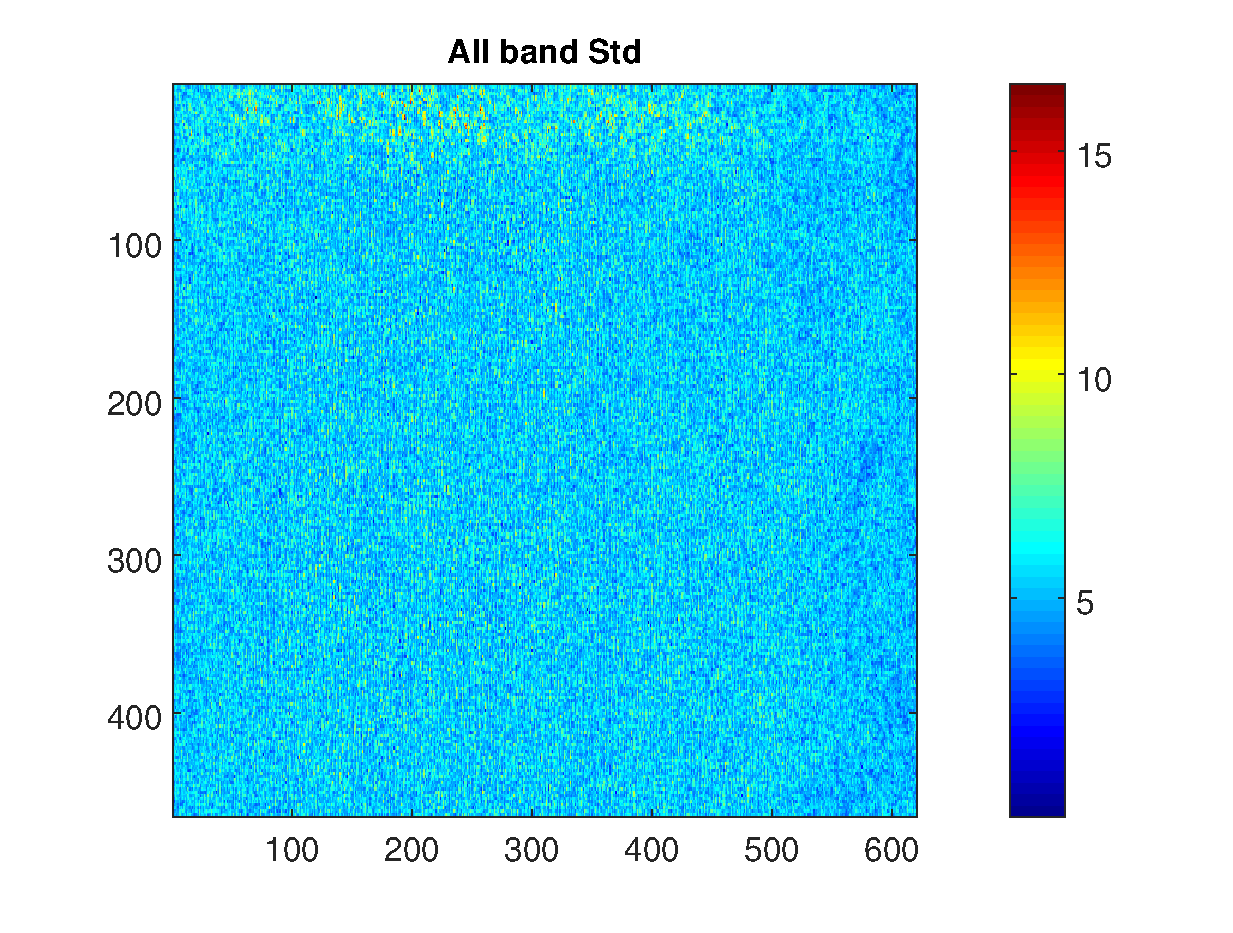
\includegraphics[width=\textwidth]{stdall.eps}
	\caption{$\sigma_T$ matrix over the complete frequency band.}
        \label{fig:papelall}
    \end{subfigure}
    ~
    \begin{subfigure}[b]{0.465\textwidth}
        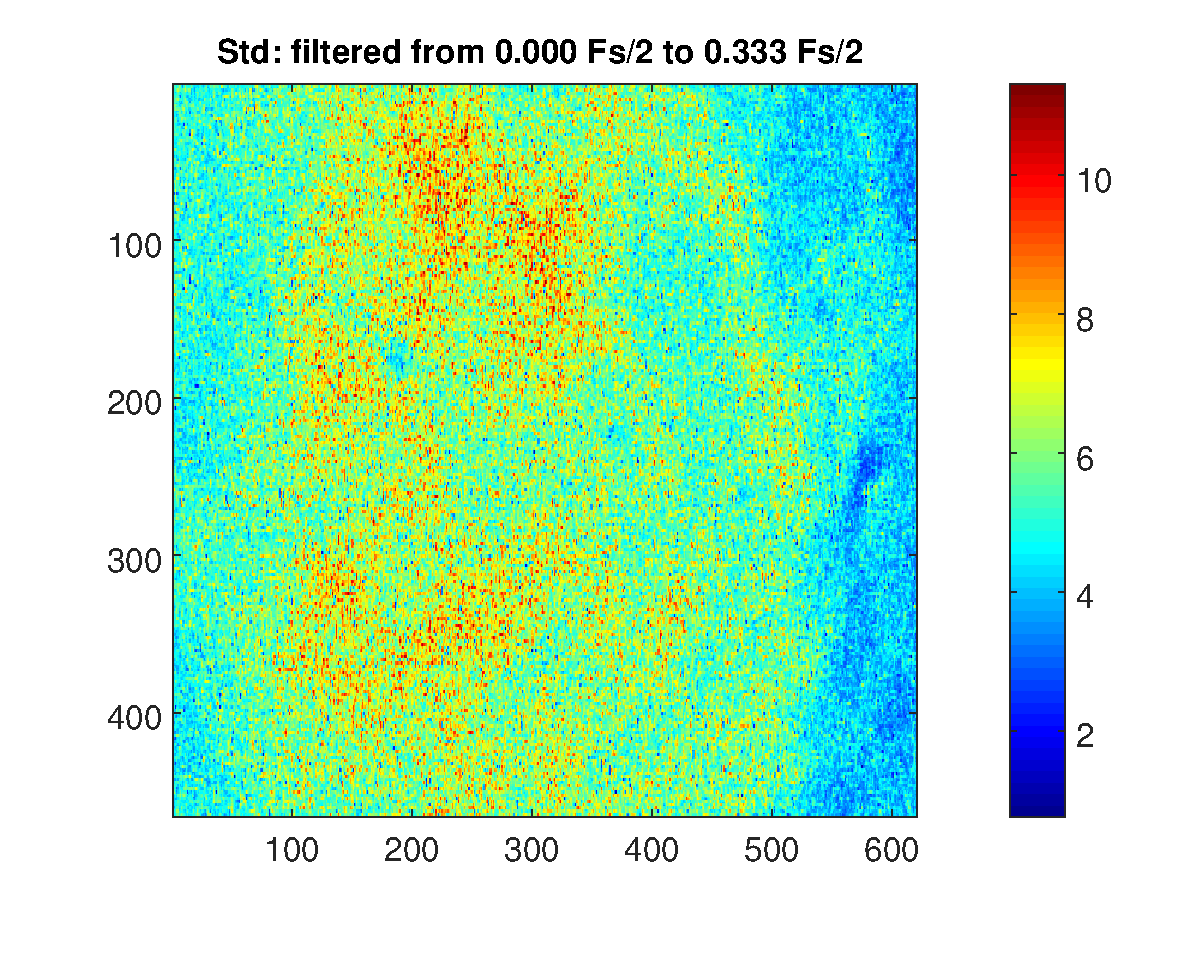
\includegraphics[width=\textwidth]{stdx.eps}
	\caption{$\sigma_X$ matrix over the inferior third of the frequency band.}
        \label{fig:papelstd_stdx}
    \end{subfigure}
    ~\\ 
    \begin{subfigure}[b]{0.475\textwidth}
        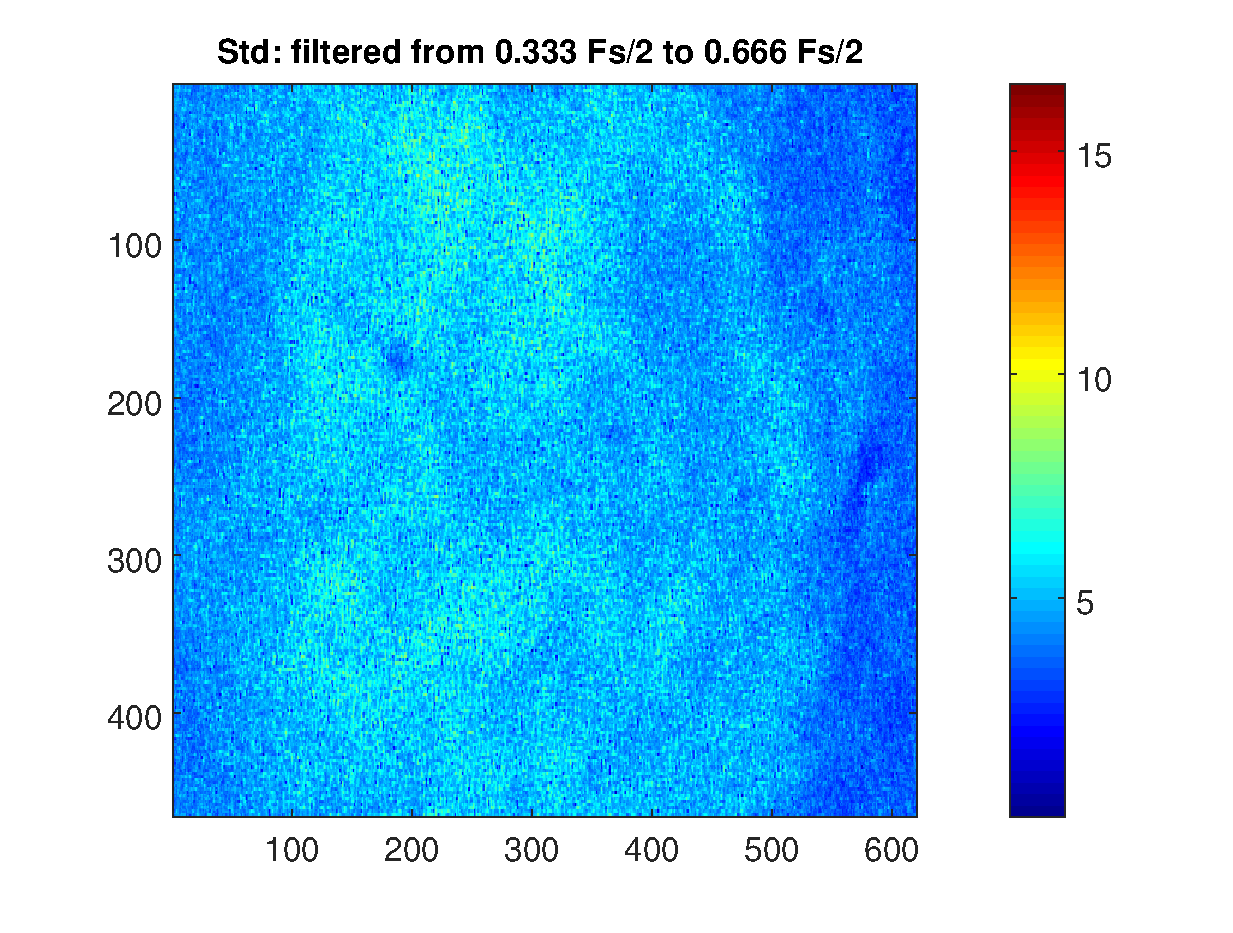
\includegraphics[width=\textwidth]{stdy.eps}
	\caption{$\sigma_Y$ matrix over the middle third of the frequency band.}
        \label{fig:papelstd_stdy}
    \end{subfigure}
  ~
    \begin{subfigure}[b]{0.475\textwidth}
        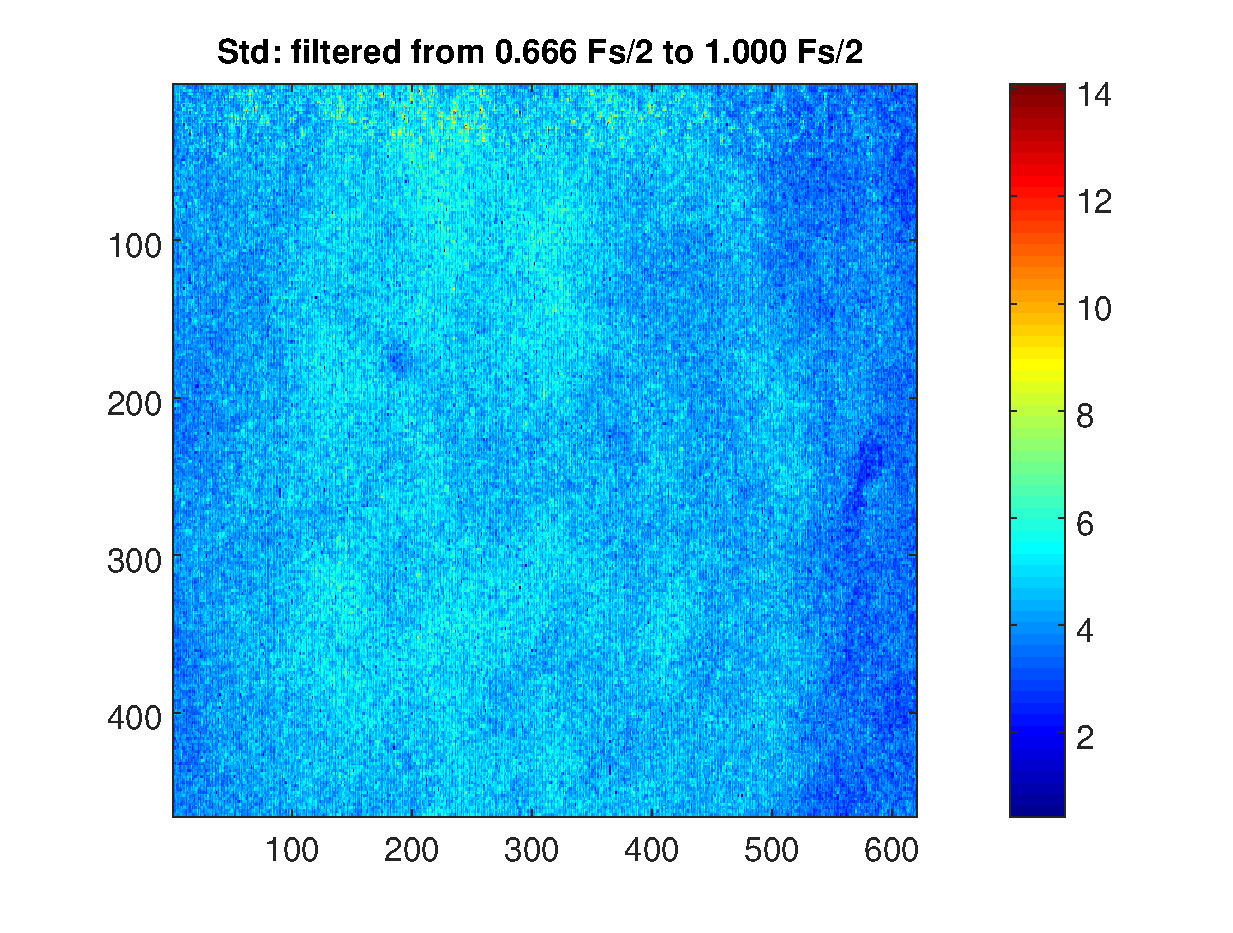
\includegraphics[width=\textwidth]{stdz.eps}
	\caption{$\sigma_Z$ matrix over the superior third of the frequency band.}
        \label{fig:papelstd_stdz}
    \end{subfigure}
    
    \caption{Temporal speckle deviation matrix of paper piece.}
    \label{fig:papelstd}
\end{figure}


In Fig. \ref{fig:papelilllevel} we present the relation between an average value of $\sigma_p$,
in the $\sigma$ matrix, with a value $\mu_p$ (mean value representing the observable illumination level) of the $\mu$ matrix, 
in the complete frequency band, the value $\mu_p$
is related to the laser illumination level in the surface of the sample \cite{Nothdurft:05}
and the color of it. Thus, when we choose $\mu_p$  as reference 
in a homogeneous sample,  
in true we choose indirectly the observable illumination level in the surface.
Therefore, Fig. \ref{fig:papelilllevel} shows the variables $\sigma_p$, $e_p$ and $L_p$ in function
of  $\mu_p$, to the case of the complete frequency band (\ref{fig:illlevel_all}), 
the inferior third of the frequency band (\ref{fig:illlevel_stdx}),
the middle third of the frequency band (\ref{fig:illlevel_stdy}) 
and the superior third of the frequency band (\ref{fig:illlevel_stdz}). 
It is import to note that $e_p$ was plot as a relation of $\sigma_p$, this means  $100 \frac{e_p}{\sigma_p} \%$,
and $L_p$ is the histogram of the values in temporal speckle mean matrix.
Given that the mean value is zero to any frequency band without the zero frequency,
in the figures are showed the $L_p$ values of the complete frequency band, 
with the objective of to have a reference of the illumination level and the number of pixels involved in the analysis.

\begin{figure}[h!]
    \centering
    \begin{subfigure}[b]{0.475\textwidth}
        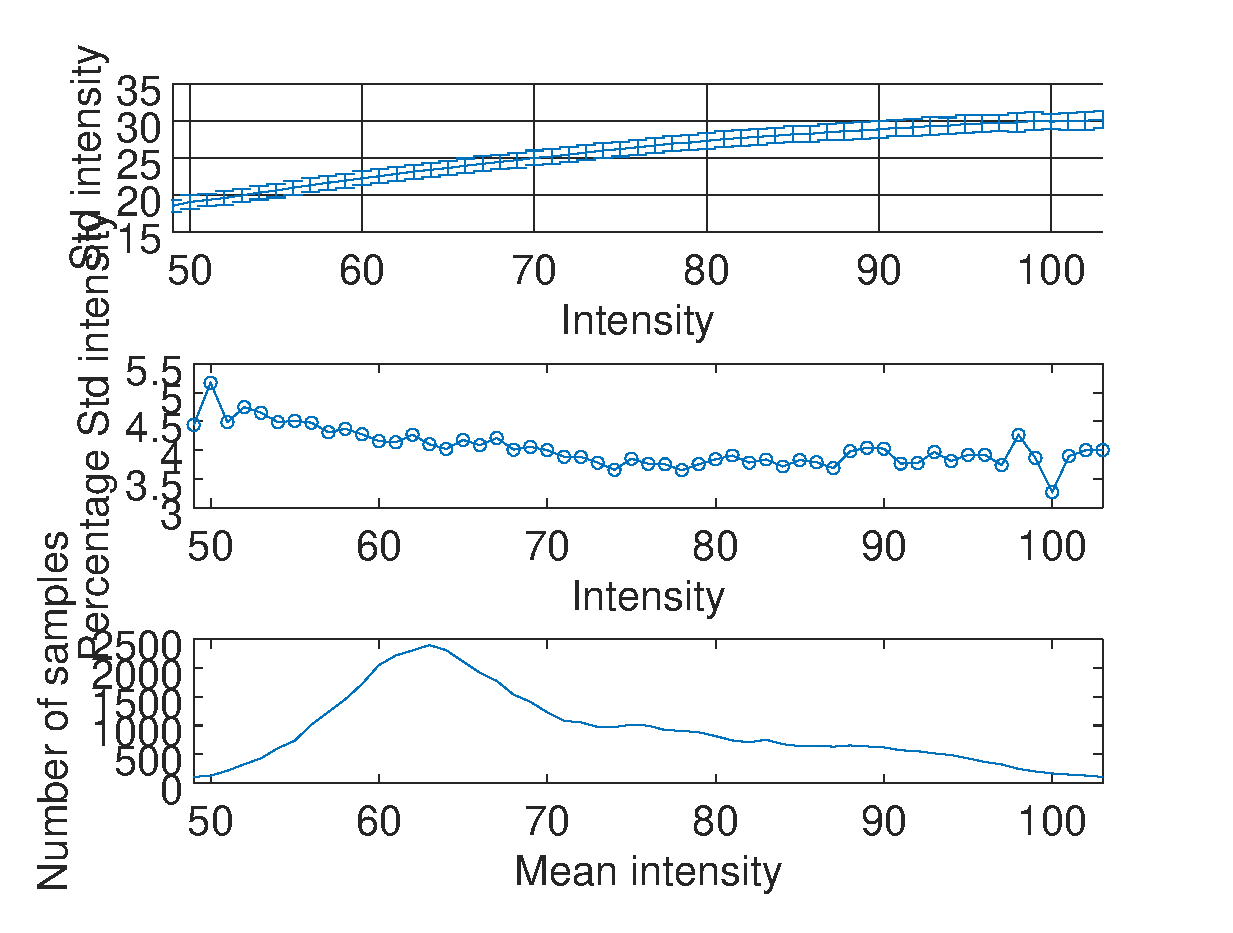
\includegraphics[width=\textwidth]{stdall_curve.eps}
	\caption{Analysis in the complete frequency band.}
        \label{fig:illlevel_all}
    \end{subfigure}
    ~
    \begin{subfigure}[b]{0.475\textwidth}
        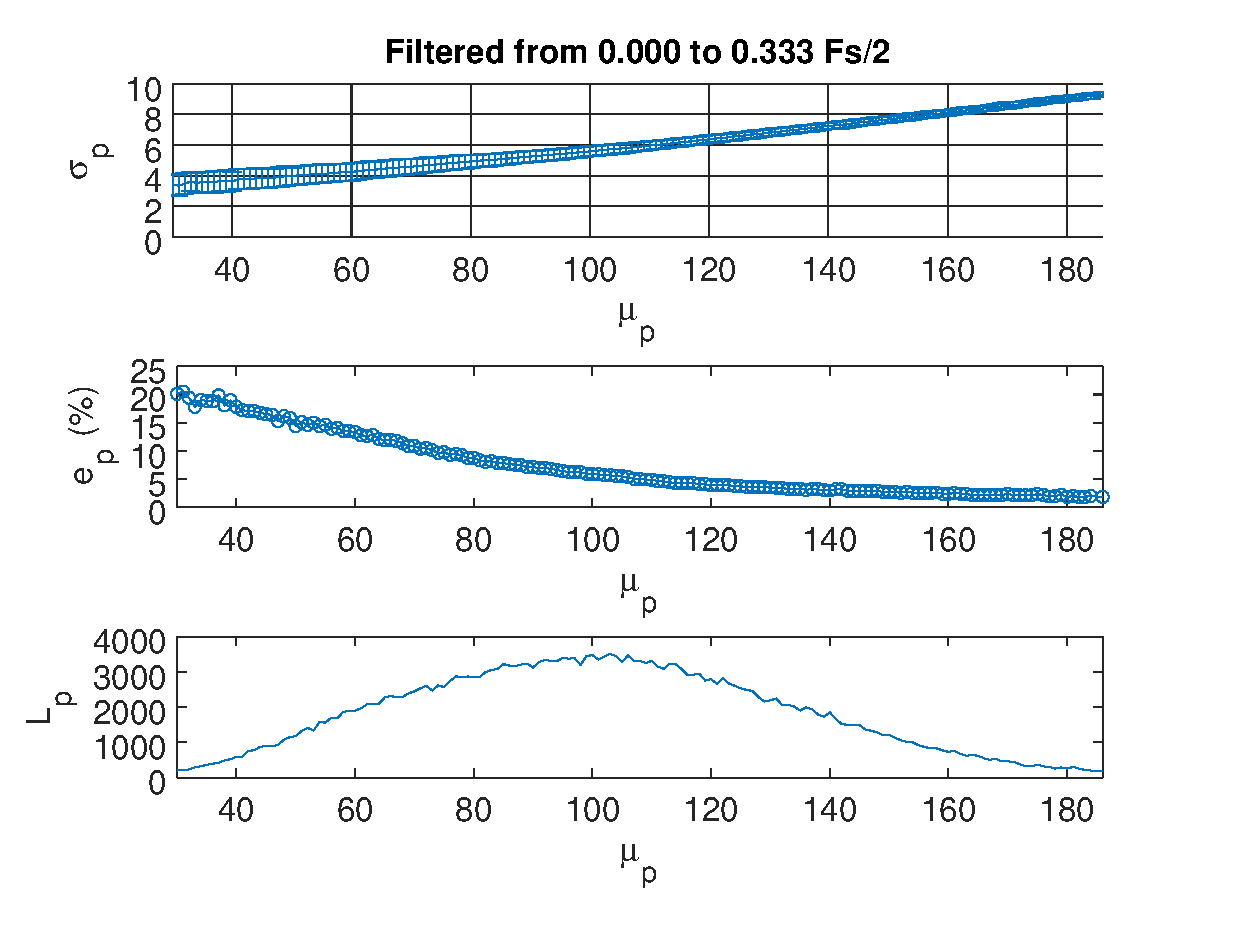
\includegraphics[width=\textwidth]{stdx_curve.eps}
	\caption{Analysis in the inferior third of the frequency band.}
        \label{fig:illlevel_stdx}
    \end{subfigure}
    ~\\ 
    \begin{subfigure}[b]{0.475\textwidth}
        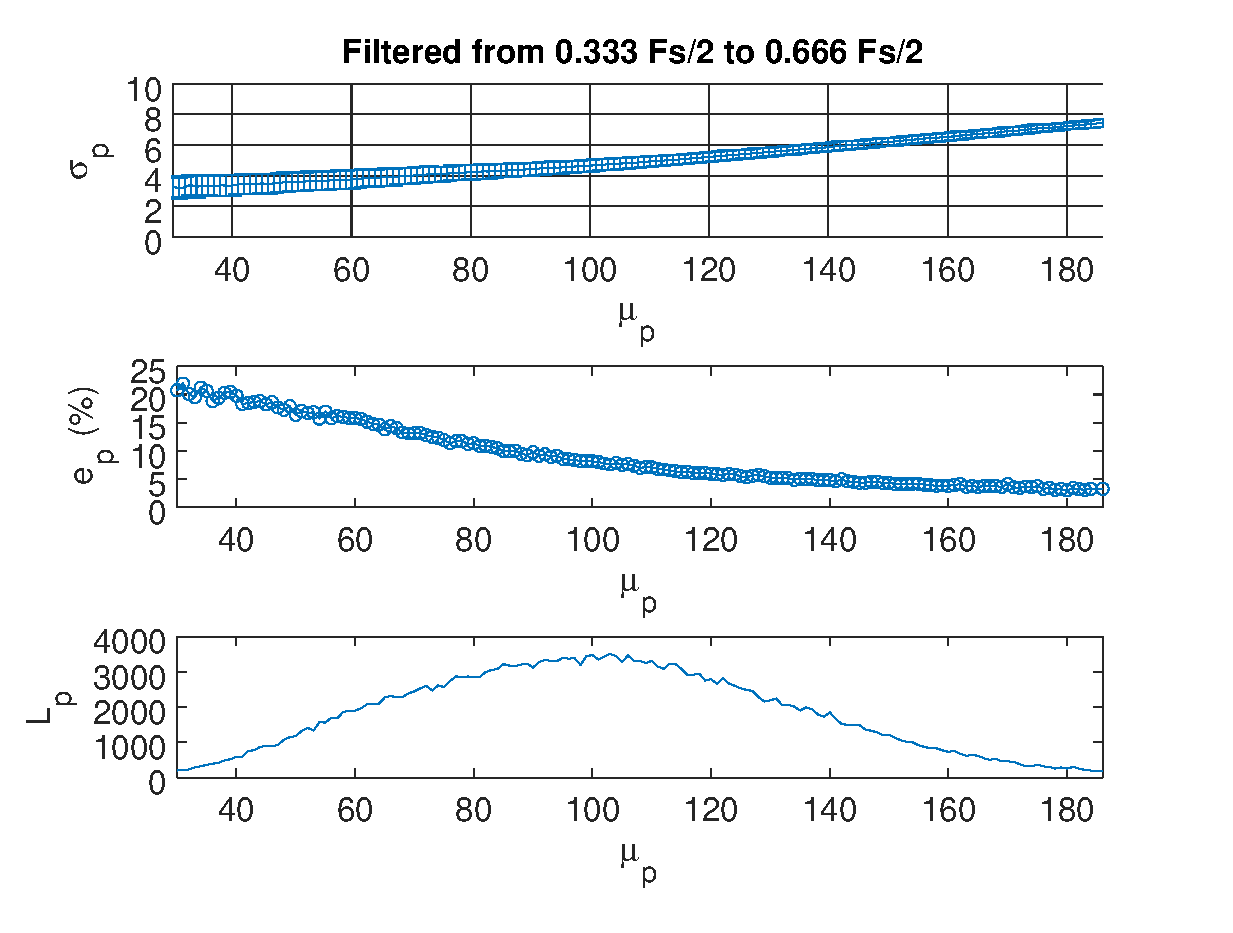
\includegraphics[width=\textwidth]{stdy_curve.eps}
	\caption{Analysis in the middle third of the frequency band.}
        \label{fig:illlevel_stdy}
    \end{subfigure}
  ~
    \begin{subfigure}[b]{0.475\textwidth}
        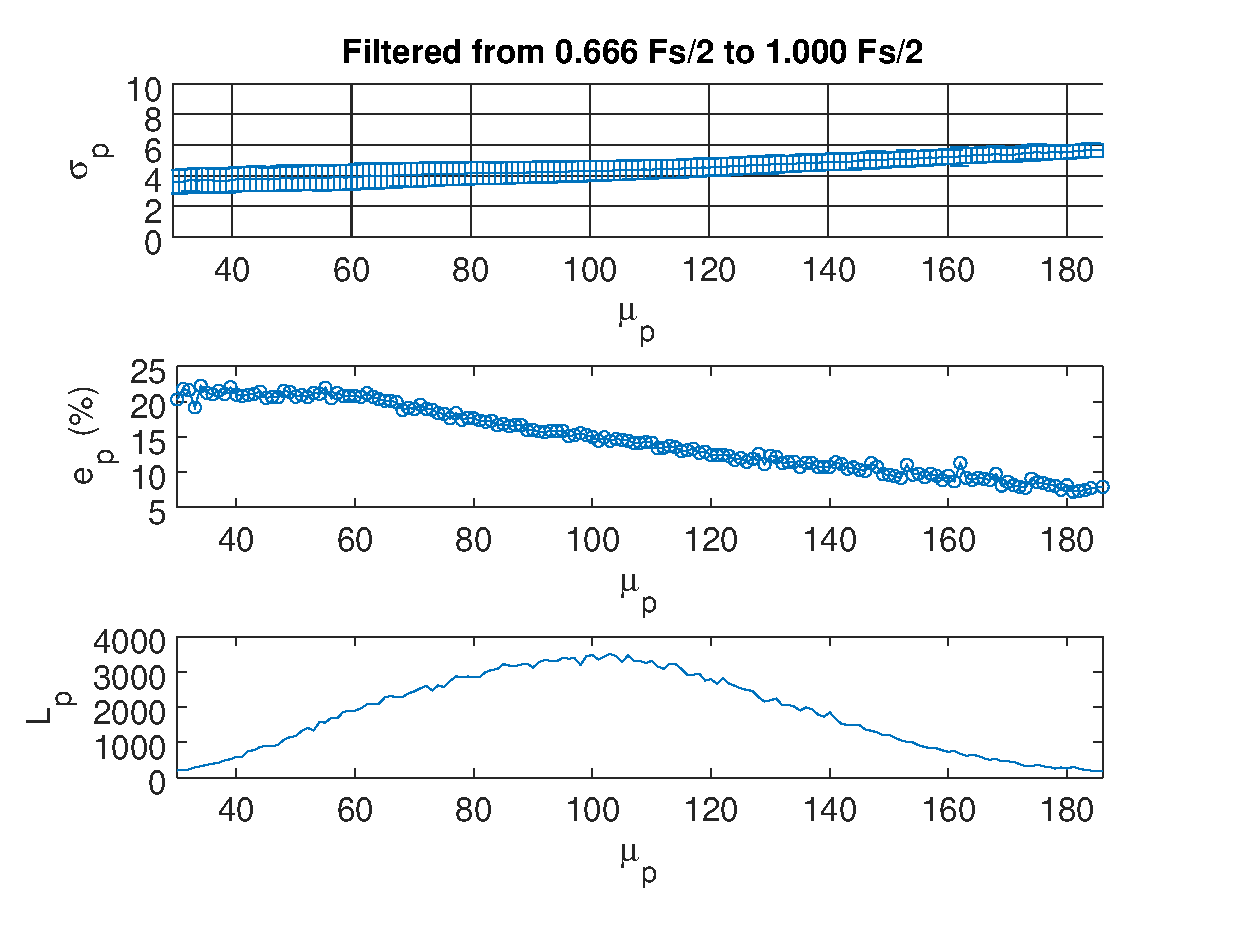
\includegraphics[width=\textwidth]{stdz_curve.eps}
	\caption{Analysis in the superior third of the frequency band.}
        \label{fig:illlevel_stdz}
    \end{subfigure}
    
    \caption{Relation between the standard deviation value and the illumination level in a steady paper under laser illumination.}
    \label{fig:papelilllevel}
\end{figure}

In Fig. \ref{fig:illlevel_all}, we observe the absence of tendency in the DLSI ($\sigma$) 
with respect to the intensity ($\mu$), 
i.e. with the increase of the $\mu$ value the standard deviation ($\sigma$) does not increase or decrease. 
However, around that constant there is a spread of $\sigma$ to each value of $\mu$ that creates an uncertainty in the outcome, 
and expressed by the error $e$. 
Fig. \ref{fig:illlevel_all} represents the outcome from the data without filtering, thus with all frequencies. 
And the data are the speckle signals present in a material with low activity, 
because the sample is a steady paper approximately homogeneous over time and space.
Nevertheless, when we filter the signal (images in time), 
we can observe a change in the $\sigma$ with respect to the frequency range, 
unveiling the dependency of the DLSI to the level of illumination and its relation to the frequency.
In Fig. \ref{fig:illlevel_stdx}, corresponding to the inferior third of the frequency band, 
there is a tendency in the $\sigma$ value with respect to the level of light. 
The DLSI changes its value with respect to the illumination level $\mu_p$, 
where in low illumination level we had highest error, 
%with the $\sigma$ values spread around the mean value, 
and the error tending to zero when the level of light ($\mu_p$) increased in some areas of the sample. 
The same behavior happened in the middle level of frequency band, 
and much less in the superior third of the frequency band, 
meaning that in the highest frequencies one had less influence of the level of light ($\mu_p$) in the $\sigma$ values. 
Since the $\sigma$ DLSI does not filter the signal \cite{RIVERA2017144}, 
it must be considered this situation during the usage of any DLSI, 
and of how this one can compromise the outcome by the influence of the illumination of the sample in the results.
Other dynamic laser speckle indexes may offer other options to avoid this influence,
for example, using the Absolute Value of the Differences DLSI and its variations \cite{BSLTLBOOK}.

\subsection{Fujii index in the ink drying test} 
\label{subsec:vsfujii}

The Fig. \ref{fig:fujiiallink} shows the behavior of mean value to the Fujii matrix
defined in the Equation \ref{eq:contFujii2}.
The Figs. \ref{fig:fujiixink}, \ref{fig:fujiiyink} and \ref{fig:fujiizink},
show the behavior of mean value to the Fujii matrix defined in the Equation \ref{eq:contFujii3},
to the cases of frequency bands X,Y and Z respectively. In all cases we worked on the ink drying test.
\begin{figure}[!h]
    \centering
    \begin{subfigure}[b]{0.475\textwidth}
        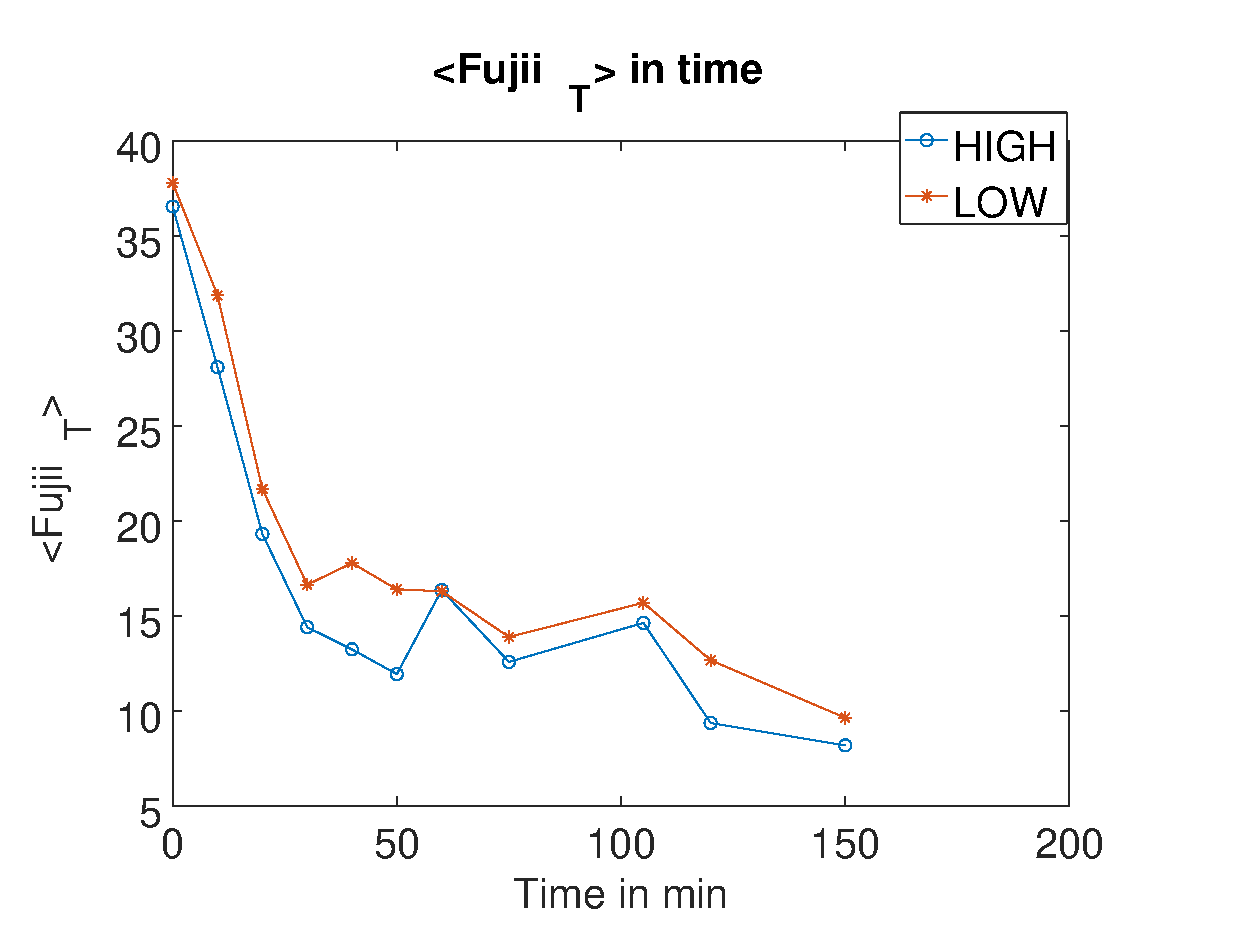
\includegraphics[width=\textwidth]{fujii-all.eps}
	\caption{Fujii value in the complete band.}
        \label{fig:fujiiallink}
    \end{subfigure}
    ~
    \begin{subfigure}[b]{0.475\textwidth}
        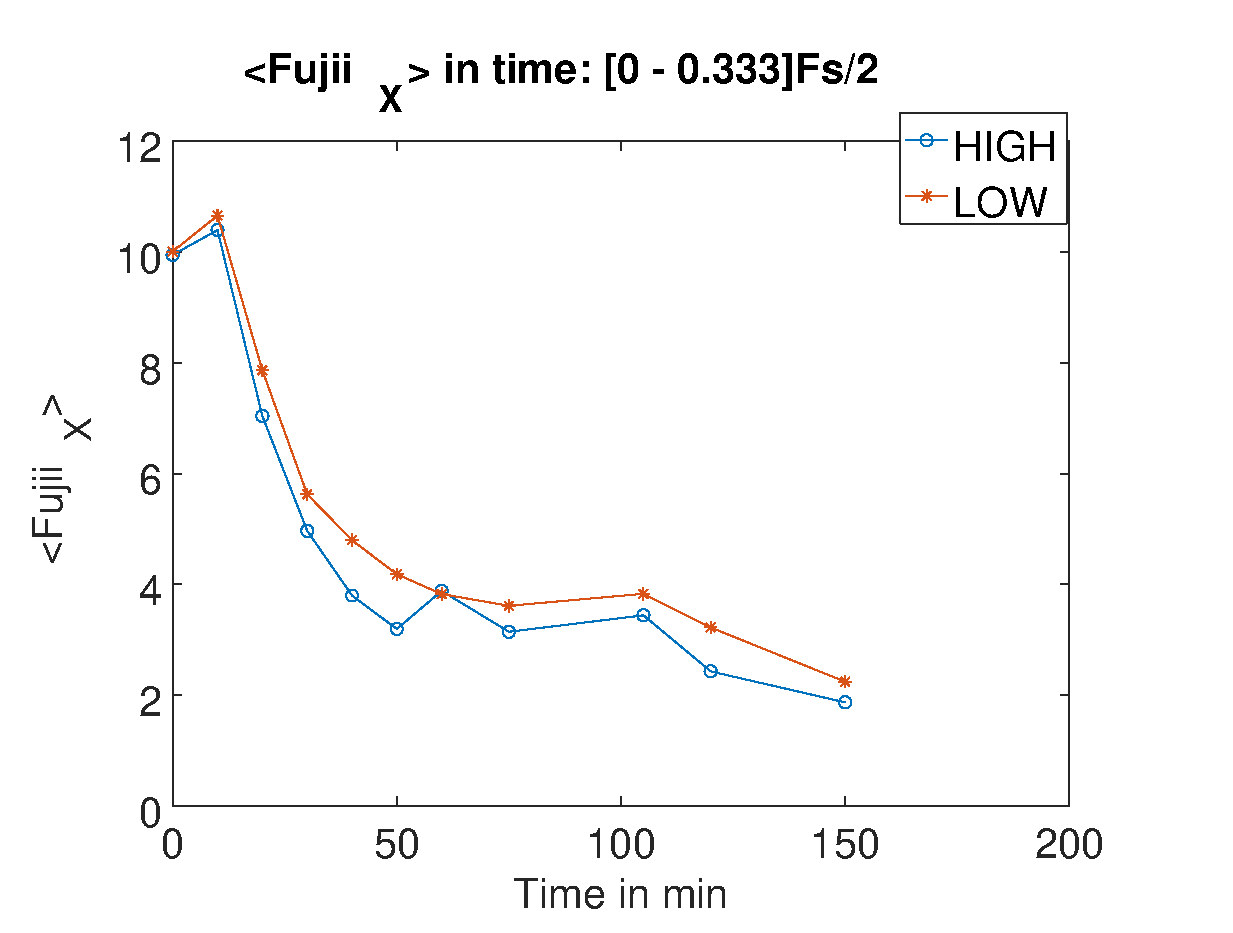
\includegraphics[width=\textwidth]{fujii-bandx.eps}
	\caption{Fujii value in the X band.}
        \label{fig:fujiixink}
    \end{subfigure}
    ~\\ 
    \begin{subfigure}[b]{0.475\textwidth}
        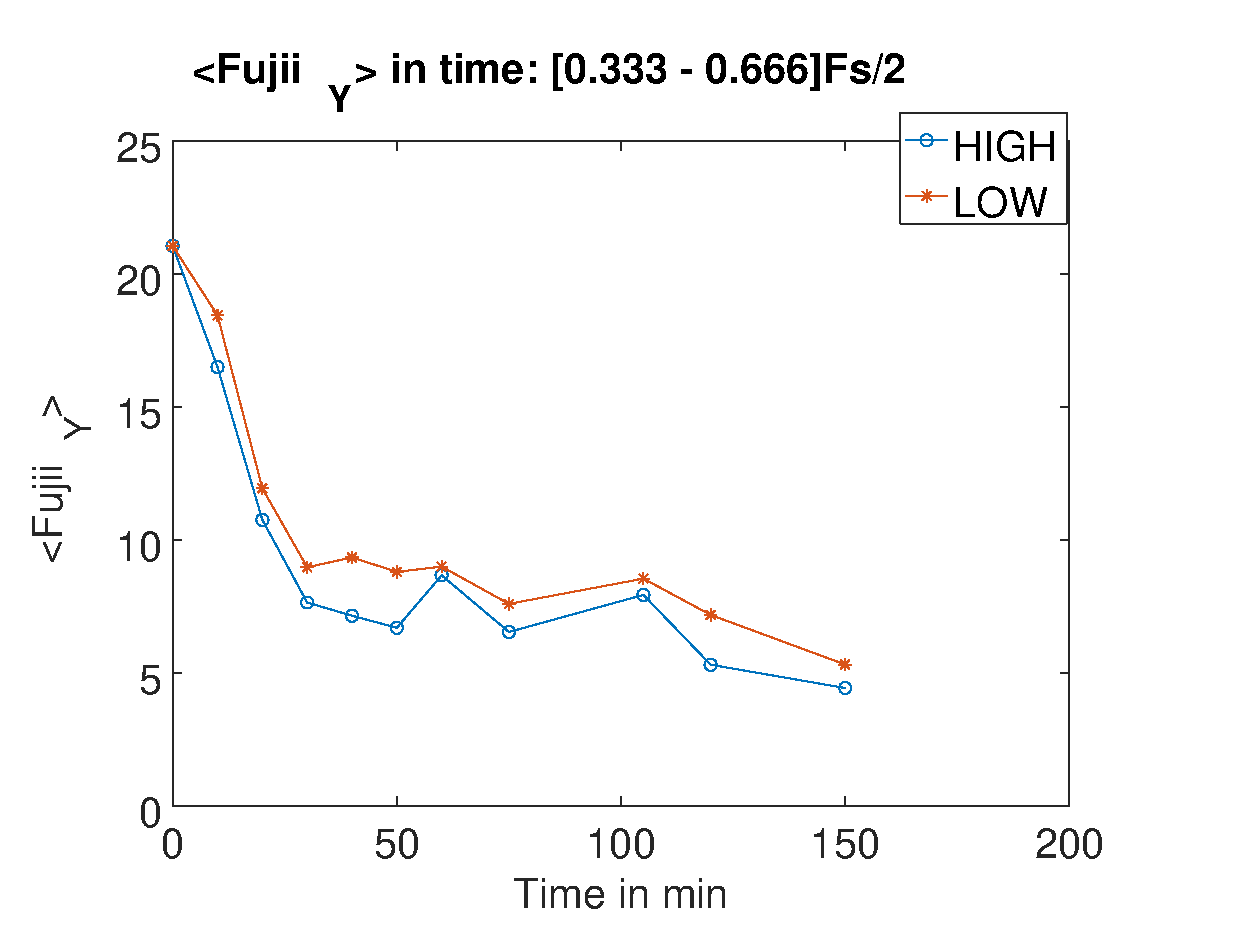
\includegraphics[width=\textwidth]{fujii-bandy.eps}
	\caption{Fujii value in the Y band.}
        \label{fig:fujiiyink}
    \end{subfigure}
  ~
    \begin{subfigure}[b]{0.475\textwidth}
        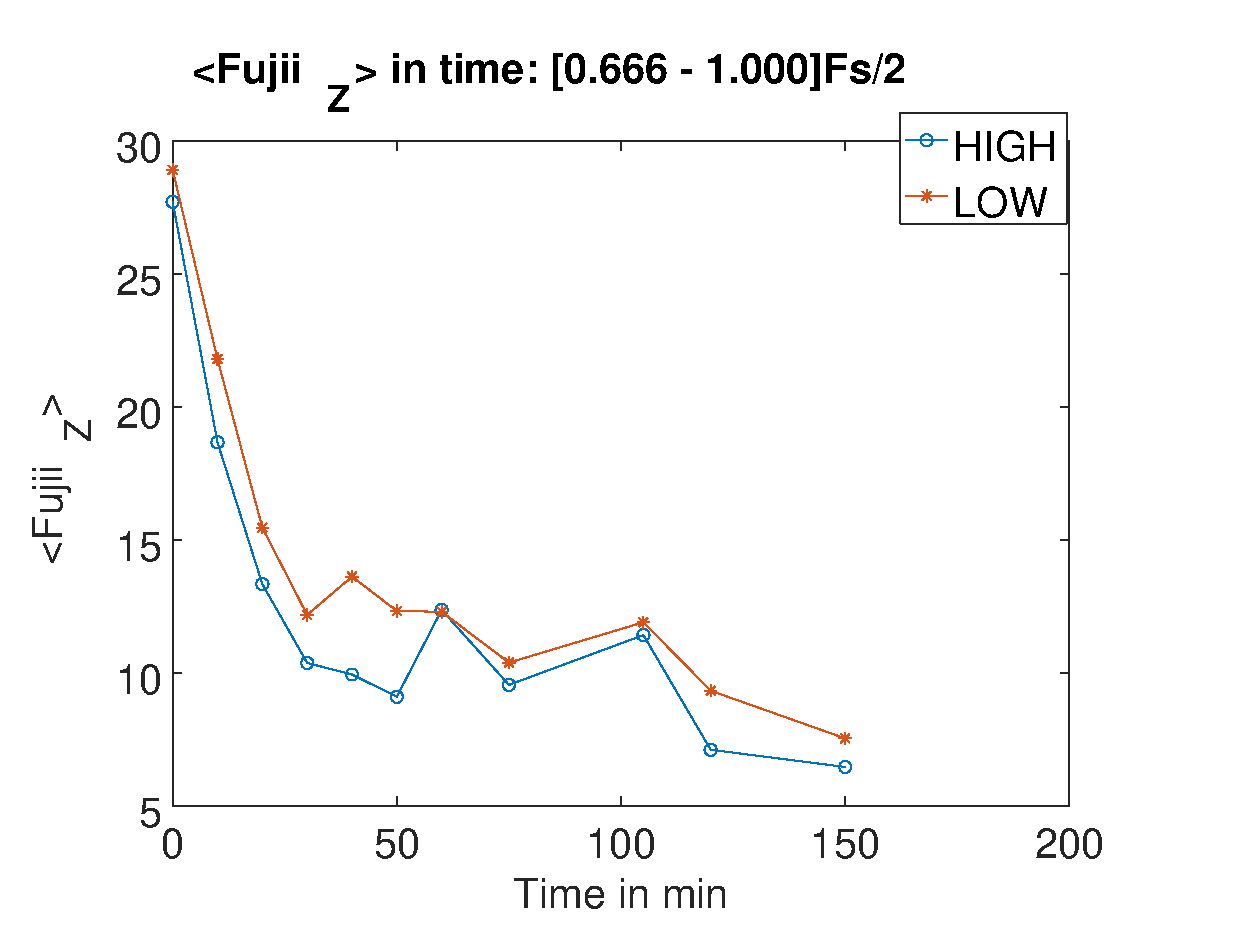
\includegraphics[width=\textwidth]{fujii-bandz.eps}
	\caption{Fujii value in the Z band.}
        \label{fig:fujiizink}
    \end{subfigure}
    
\caption{Numerical results in the ink drying test using Fujii index.}
\label{fig:numericalvsfujii}
\end{figure}

As can be seen in all the images, the curves with more and less  illumination level are close,
but there is no advantage in separating the signals by bands
this can be explained if we analyze how the index synthesizes its value and we compares it with the images.
First the Fujii index makes a high pass filtering,
this is evident if we look at the maximum values of the curves,
being greater in the Z (high frequencies) band and rapidly decrease in the Y and X (low frequencies) bands.
Second, the index undergoes a normalization, in the denominator of the Equation \ref{eq:contFujii2},
with the intention of reducing the index dependence with the sample level of illumination.
Not to mention that this normalization, in the case of frequency band analysis, is done with unfiltered signal data.

%%%%%%%%%%%%%%%%%%%%%%%%%%%%%%%%%%%%%%%%%%%%%%%%%%%%%%%%%%%%%%%%%%%%%%%%%%%%%%%%%%%%%%%%%
%%%%%%%%%%%%%%%%%%%%%%%%%%%%%%%%%%%%%%%%%%%%%%%%%%%%%%%%%%%%%%%%%%%%%%%%%%%%%%%%%%%%%%%%%
\section{Final comments} 

By the results shown in the Figs. \ref{fig:numerical} and \ref{fig:papelilllevel},
we can theorize that the dynamic range,
between the samples with greater and  less values, 
in  the temporal speckle deviation index,
they are greater on speckle signals with low frequency components, 
and  smaller on speckle signals with high frequency components;
thus, we can observe that the effect of illumination level in 
the variability of the temporal speckle deviation index decrease with the frequency.
This hypothesis is supported by other works with similar results \cite{Nothdurft:05},
where the temporal speckle mean matrix shows information about the surface of sample and the laser illumination level, 
and the temporal speckle deviation matrix shows information of material inside at 
different levels and in less proportion the information of the laser illumination level.
Given that the mean value collect information of zero frequency component in the speckle signal, 
and the standard deviation  collect information of non-zero frequency components.
We can make a parallel, 
with the results obtained in the present work,
and thus  to indicate that the speckle signals with high frequency components
 are less affected in their dynamic range by the variation of the laser light intensity.
By analyzing the index Fujii, 
we also highlight that generalizations cannot be made for all speckle indices.
In this work we mainly use the standard deviation, because its calculation is directly linked to the value, 
or amplitude, root mean square of the signals.
In counter-parted, the Fujii index makes a previous filtering (subtract a sample with the previous one) 
and a non-linear scaling with respect to the light intensity (divide by the average intensity between two consecutive samples), 
which hinders a fair interpretation, of its behavior for different frequency bands.


%%%%%%%%%%%%%%%%%%%%%%%%%%%%%%%%%%%%%%%%%%%%%%%%%%%%%%%%%%%%%%%%%%%%%%%%%%%%%%%%%%%%%%%%%
%%%%%%%%%%%%%%%%%%%%%%%%%%%%%%%%%%%%%%%%%%%%%%%%%%%%%%%%%%%%%%%%%%%%%%%%%%%%%%%%%%%%%%%%%
\section{Conclusion} 

In the ink drying test, 
we analyzed a process that changes its behavior over time,
and we seen the effect produced in  the speckle light intensity, 
and consequently in the standard deviation index, 
by the separation of the signals in different frequency bands.
By other side, in the paper piece test, 
we considered that none material is completely inert and, consequently, 
the observed signal  in the  dynamic speckle analysis has more than noise.

%% Mayor quantidade de luz, mayor sigma index
By the analysis of paper piece shown in the Figs. \ref{fig:illlevel_stdx}, \ref{fig:illlevel_stdy} and \ref{fig:illlevel_stdz};
we can see that the greater the observable laser illumination level $\mu_p$, 
the greater will the $\sigma_p$ index of each pixel analyzed, 
however this increase depend of frequency band in the speckle signal  analyzed;
by example, in the Fig. \ref{fig:illlevel_stdz},
with high frequency components, the relation between $\mu_p$ and $\sigma_p$ its almost a horizontal line, 
this mean that the variation of $\mu_p$ no affect significantly to the $\sigma_p$ index.
This is reaffirmed by the analysis of the ink drying test, 
seen in the Figs. \ref{fig:stdxink}, \ref{fig:stdyink} and \ref{fig:stdzink},
where the curves of regions with high and low luminosity are compared in different frequency bands,
being the case with high frequency band  (Fig. \ref{fig:stdzink}) 
the one that produces very similar indices, despite the difference in the illumination level.


Thus, in this work were presented comparisons between the values of the temporal 
speckle deviation index for three different frequency bands of the speckle signal and 
different illuminations levels in a dynamic laser speckle analysis. 
The results showed that the influence of the observable illumination level in a DLSI, 
like the temporal speckle deviation index, 
decreases with the use of signals with high frequency components.


\section{Acknowledgment}
We wish to acknowledge the partial financial support for this study provided by the $CAPES$ 
scholarship
$PNPD$ Program, $FAPEMIG$ and $CNPQ$.

%----------------------------------------------------------------------------------------
%	REFERENCE LIST
%----------------------------------------------------------------------------------------
\section{Bibliography}
\bibliography{report}   %>>>> bibliography data in report.bib
\bibliographystyle{spiebib}   %>>>> makes bibtex use spiebib.bst


%----------------------------------------------------------------------------------------

\end{document} 


